\documentclass{article}

\usepackage[preprint]{corl_2021} % Use this for the initial submission.
%\usepackage[final]{corl_2021} % Uncomment for the camera-ready ``final'' version.
%\usepackage[preprint]{corl_2021} % Uncomment for pre-prints (e.g., arxiv); This is like ``final'', but will remove the CORL footnote.
\usepackage{enumitem}
\usepackage{graphicx}
\usepackage{booktabs}
\usepackage{xcolor}
\usepackage{amsmath,units}
\usepackage{amssymb}
\usepackage{comment}

\newcommand{\SE}{\mathrm{SE}}
\newcommand{\SO}{\mathrm{SO}}
\newcommand{\R}{\mathbb{R}}
\newcommand{\bb}{\boldsymbol{b}}
\newcommand{\bff}{\boldsymbol{f}}
\newcommand{\bc}{\boldsymbol{c}}
\newcommand{\bo}{\boldsymbol{o}}
\newcommand{\bp}{\boldsymbol{p}}
\newcommand{\bq}{\boldsymbol{q}}
\newcommand{\bx}{\boldsymbol{x}}
\newcommand{\bv}{\boldsymbol{v}}
\newcommand{\by}{\boldsymbol{y}}
\newcommand{\bt}{\boldsymbol{t}}
\newcommand{\bR}{\boldsymbol{R}}
\newcommand{\bH}{\boldsymbol{H}}
\newcommand{\bS}{\boldsymbol{S}}
\newcommand{\bV}{\boldsymbol{V}}
\newcommand{\bU}{\boldsymbol{U}}

\newcommand{\XY}{\mathcal{XY}}
\newcommand{\YX}{\mathcal{YX}}
\newcommand{\I}{\mathcal{I}}
\newcommand{\B}{\mathcal{B}}
\newcommand{\C}{\mathcal{C}}
\newcommand{\T}{\mathcal{T}}


\newcommand{\OO}{\mathcal{O}}
\newcommand{\Q}{\mathcal{Q}}
\newcommand{\X}{\mathcal{X}}
\newcommand{\Y}{\mathcal{Y}}
\newcommand{\F}{\mathcal{F}}
\newcommand{\N}{\mathcal{N}}
\newcommand{\A}{\mathcal{A}}
\newcommand{\avg}{\mathrm{avg}}
\DeclareMathOperator*{\argmax}{arg\,max}
\DeclareMathOperator*{\argmin}{arg\,min}
\newcommand{\justin}[1]{\textbf{\scriptsize{\color{red}JS: #1}}}
\newcommand{\vitor}[1]{\textbf{\scriptsize{\color{blue}VG: #1}}}
\newcommand{\yue}[1]{\textbf{\scriptsize{\color{green}YW: #1}}}
\newcommand{\tianyuan}[1]{\textbf{\scriptsize{\color{yellow}TYZ: #1}}}
\newcommand{\changed}[1]{{\color{black}{#1}}}

\newcommand{\name}{DETR3D }

\setlist{noitemsep,leftmargin=*}

% \title{MVDet:\\ Multi-view Object Detection via Set-to-Set Prediction}
\title{DETR3D：通过3D到2D查询实现多视角图像3D目标检测（3D Object Detection from Multi-view Images via 3D-to-2D Queries）}

% The \author macro works with any number of authors. There are two
% commands used to separate the names and addresses of multiple
% authors: \And and \AND.
%
% Using \And between authors leaves it to LaTeX to determine where to
% break the lines. Using \AND forces a line break at that point. So,
% if LaTeX puts 3 of 4 authors names on the first line, and the last
% on the second line, try using \AND instead of \And before the third
% author name.

% NOTE: authors will be visible only in the camera-ready and preprint versions (i.e., when using the option 'final' or 'preprint'). 
% 	For the initial submission the authors will be anonymized.

\author{
  Yue Wang\\
  Massachusetts Institute of Technology \\
  \texttt{yuewang@csail.mit.edu} \\
  %% examples of more authors
   \And
  Vitor Guizilini* \\ 
  Toyota Research Institute \\ 
  \texttt{vitor.guizilini@tri.global} \\
  \And 
  Tianyuan Zhang* \\ 
  Carnegie Mellon University \\
  \texttt{tianyuaz@andrew.cmu.edu} \\
  \And 
  Yilun Wang \\ 
  Li Auto \\ 
  \texttt{yilunw@cs.stanford.edu} \\
  \And
  Hang Zhao $\P$ \\ 
  Tsinghua University \\ 
  \texttt{hangzhao@mail.tsinghua.edu.cn} \\
  \And
  Justin Solomon $\P$ \\
  Massachusetts Institute of Technology \\
  \texttt{jsolomon@mit.edu}
}




% Chinese support (auto-injected)
\usepackage{xeCJK}
\setCJKmainfont{Noto Serif CJK SC}[ItalicFont=AR PL UKai TW MBE]
\setCJKsansfont{Noto Sans CJK SC}
\setCJKmonofont{Noto Sans CJK SC}
\raggedbottom
\renewcommand{\figurename}{图}
\renewcommand{\tablename}{表}
\renewcommand{\abstractname}{摘要}
\renewcommand{\refname}{参考文献}
\begin{document}
\maketitle
\let\thefootnote\relax\footnotetext{*: 同等贡献（Equal contribution）。$\P$: 项目共同指导（Co-advise）。}


%===============================================================================
\begin{abstract}
本文提出了一种多相机3D目标检测（Multi-Camera 3D Object Detection）框架。
与直接从单目图像估计3D边界框或使用深度预测网络从2D信息生成3D目标检测输入的现有方法不同，本文方法直接在3D空间中进行预测。本文架构从多个相机图像中提取2D特征，然后使用稀疏的3D目标查询集合索引这些2D特征，通过相机变换矩阵将3D位置与多视角图像关联起来。最终，本文模型对每个目标查询进行边界框预测，并使用集合到集合（Set-to-Set）损失来衡量预测与真值之间的差异。
本文研究了连接2D观测与3D预测的两种方案：一种是依赖于密集深度预测和3D场景结构恢复的自底向上（Bottom-Up）方法；另一种是从稀疏目标先验出发，通过反向投影（Backward Projection）查询2D图像特征的自顶向下（Top-Down）方法。
这种自顶向下方法优于自底向上方法（后者在逐像素深度估计后进行目标边界框预测），因为它不受深度预测模型引入的累积误差影响。此外，本文方法不需要非极大值抑制（Non-Maximum Suppression, NMS）等后处理，显著提升了推理速度。本文在nuScenes自动驾驶基准上取得了当前最优（State-of-the-Art, SOTA）的性能。
\end{abstract}


\section{引言}

从视觉信息中进行3D目标检测（3D Object Detection）一直是低成本自动驾驶系统面临的长期挑战。虽然利用激光雷达（LiDAR）等传感器采集的点云进行目标检测得益于可见物体3D结构信息，但基于相机的设置更为不适定，因为必须仅从RGB图像中包含的2D信息生成3D边界框预测。

现有方法~\cite{zhou2019centernet,wang2021fcos3d}通常完全基于2D计算构建检测流程。它们使用为2D任务设计的检测流程（如CenterNet~\cite{zhou2019centernet}、FCOS~\cite{tian2019fcos}）来预测物体姿态和速度等3D信息，而未考虑3D场景结构或传感器配置。这些方法需要多个后处理步骤来融合不同相机的预测并去除冗余边界框，导致效率和效果之间存在严重权衡。

作为这些基于2D方法的替代方案，一些方法通过应用3D重建方法~\cite{monodepth2,bts,packnet}，从相机图像创建场景的伪激光雷达（Pseudo-LiDAR）或距离输入，从而将更多3D计算引入检测流程。然后，可对这些数据应用3D目标检测方法，就像直接来自3D传感器一样。然而，这种策略会受到累积误差的影响~\cite{demistifying}：估计不准确的深度值会对3D目标检测性能产生强烈的负面影响，而3D目标检测本身也可能产生误差。

本文提出了一种更优雅的2D观测与3D预测之间的转换方案，该方案不依赖密集深度预测模块。本文框架称为\name（多视角3D检测），以自顶向下的方式解决该问题。通过几何反向投影（Geometric Back-Projection）和相机变换矩阵，将2D特征提取与3D目标预测相连接。

本文方法从一组稀疏的目标先验开始，这些先验在数据集上共享并以端到端方式学习。为获取场景特定信息，将从这些目标先验解码得到的一组参考点反向投影到每个相机，并获取由ResNet骨干网络~\cite{He2015}提取的相应图像特征。参考点的图像特征随后通过多头自注意力层~\cite{Vaswani2017}进行交互。经过一系列自注意力层后，从每一层读取边界框参数，并使用受DETR~\cite{detr}启发的集合到集合损失来评估性能。

本文架构不进行点云重建或从图像显式预测深度，因此对深度估计误差具有鲁棒性。此外，本文方法不需要任何后处理（如非极大值抑制），提高了效率并减少了对人工设计的输出清洗方法的依赖。在nuScenes数据集上，本文方法（无NMS）与先前方法（有NMS）性能相当。在相机重叠区域，本文方法显著优于其他方法。

\textbf{贡献。} 本文的主要贡献总结如下：
\begin{itemize}
  \item 提出了一种基于RGB图像的简洁3D目标检测模型。与现有在最后阶段才融合不同相机视图目标预测的方法不同，本文方法在每一层计算中都融合了所有相机视图的信息。据本文所知，这是首次将多相机检测视为3D集合到集合预测的尝试。
  \item 引入了一个通过几何反向投影连接2D特征提取和3D边界框预测的模块。该模块不受辅助网络不准确深度预测的影响，并通过将3D信息反向投影到所有可用帧上无缝利用多相机信息。
  \item 与Object DGCNN~\cite{objdgcnn}类似，本文方法不需要逐图像或全局NMS等后处理，性能与现有基于NMS的方法相当。在相机重叠区域，本文方法以显著优势优于其他方法。
  \item 公开代码以促进可重复性和未来研究。\footnote{\url{https://github.com/WangYueFt/detr3d}}
\end{itemize}

\section{相关工作}

\textbf{2D目标检测（2D Object Detection）。} RCNN~\cite{girshick2014rcnn}开创了使用深度学习进行目标检测的先河。它将一组预选的目标候选框输入卷积神经网络（CNN），并据此预测边界框参数。尽管该方法表现出令人惊讶的性能，但由于需要对每个目标候选框执行一次卷积网络前向传播，其速度比其他方法慢一个数量级。为解决此问题，Fast RCNN~\cite{ren2015faster}引入了一个共享的可学习CNN，在单次前向传播中处理整张图像。为进一步提升性能和速度，Faster RCNN~\cite{ren2015faster}包含了一个区域提议网络（Region Proposal Network, RPN），该网络与检测网络共享全图卷积特征，从而几乎零成本地生成区域提议。Mask RCNN~\cite{he2017maskrcnn}引入了一个掩码预测分支，以实现并行实例分割。这些方法通常涉及多阶段优化，在实践中可能速度较慢。与这些多阶段方法不同，SSD~\cite{liu2016ssd}和YOLO~\cite{Redmon2015YouOL}以单次方式执行密集预测。虽然它们显著快于上述替代方案，但仍依赖NMS去除冗余框预测。这些方法相对于预定义的锚框（Anchors）预测边界框。CenterNet~\cite{zhou2019centernet}和FCOS~\cite{tian2019fcos}改变了范式，从逐锚框预测转向逐像素预测，大大简化了常见的目标检测流程。

\textbf{基于集合的目标检测（Set-based Object Detection）。} DETR~\cite{detr}将目标检测视为一个集合到集合问题。它使用Transformer~\cite{Vaswani2017}捕获特征和目标交互。DETR学习将预测结果分配给一组真值框，因此不需要后处理来过滤冗余框。然而，DETR的一个关键缺点是需要大量的训练时间。Deformable DETR~\cite{zhu2021deformable}分析了DETR收敛缓慢的原因，并提出了一种可变形自注意力模块来定位特征并加速训练。与此同时，\cite{Sun2020RethinkingTS}将DETR收敛缓慢归因于集合损失和Transformer交叉注意力机制，提出了TSP-FCOS和TSP-RCNN两种变体来克服这些问题。SparseRCNN~\cite{peize2020sparse}将集合预测融入RCNN风格的流程，性能优于多阶段目标检测且无需NMS。OneNet~\cite{peize2020onenet}研究了一个有趣的现象：密集目标检测器配备最小代价集合损失后，可实现无NMS检测。在3D领域，Object DGCNN~\cite{objdgcnn}研究了从点云进行3D目标检测。它将3D目标检测建模为动态图上的消息传递，将DGCNN框架推广到预测一组目标。与DETR类似，Object DGCNN也是无NMS的。

\textbf{单目3D目标检测（Monocular 3D Object Detection）。} 从RGB图像进行3D检测的早期方法是Mono3D~\cite{chen2016monocular}，它利用语义和形状线索，在训练时使用场景约束和额外先验从一组3D候选框中进行选择。\cite{roddick2018orthographic}使用鸟瞰视图（Bird's-Eye View, BEV）进行单目3D检测，而~\cite{mousavian20173d}利用2D检测结果，通过最小化2D-3D投影误差进行3D边界框回归。使用2D检测器作为3D计算的起点最近已成为一种标准方法~\cite{kehl2017ssd,ku2019monocular}。其他工作还探索了可微渲染~\cite{beker2020monocular}或3D关键点检测~\cite{barabanau2019monocular,liu2020smoke,zhou2019centernet}等方面的进展，以实现当前最优的3D目标检测性能。所有这些方法都是在单目设置下运行的，扩展到多相机的方式是独立处理每个视角的图像，然后在后处理阶段合并输出。
% \section{Method}
\section{多视角3D目标检测}
\subsection{概述}
\label{overview}
% Talk about the pipeline in high level and why our method is exciting. 
% We consider an application of 3D object detection where the scene geometry is missing and only 2D multi-camera images are available. This challenging problem gives rise to  . 

本文架构以一组相机（其投影矩阵已知）采集的RGB图像作为输入，输出场景中目标的3D边界框参数集合。与以往方法不同，本文基于以下几个高层次需求构建架构：
\begin{itemize}
    \item 在架构的中间计算中融入3D信息，而非仅在图像平面上执行纯2D计算。
    \item 不估计密集的3D场景几何结构，避免引入相关的重建误差。
    \item 避免NMS等后处理步骤。
\end{itemize}

\begin{figure}[t!]  
    \centering
    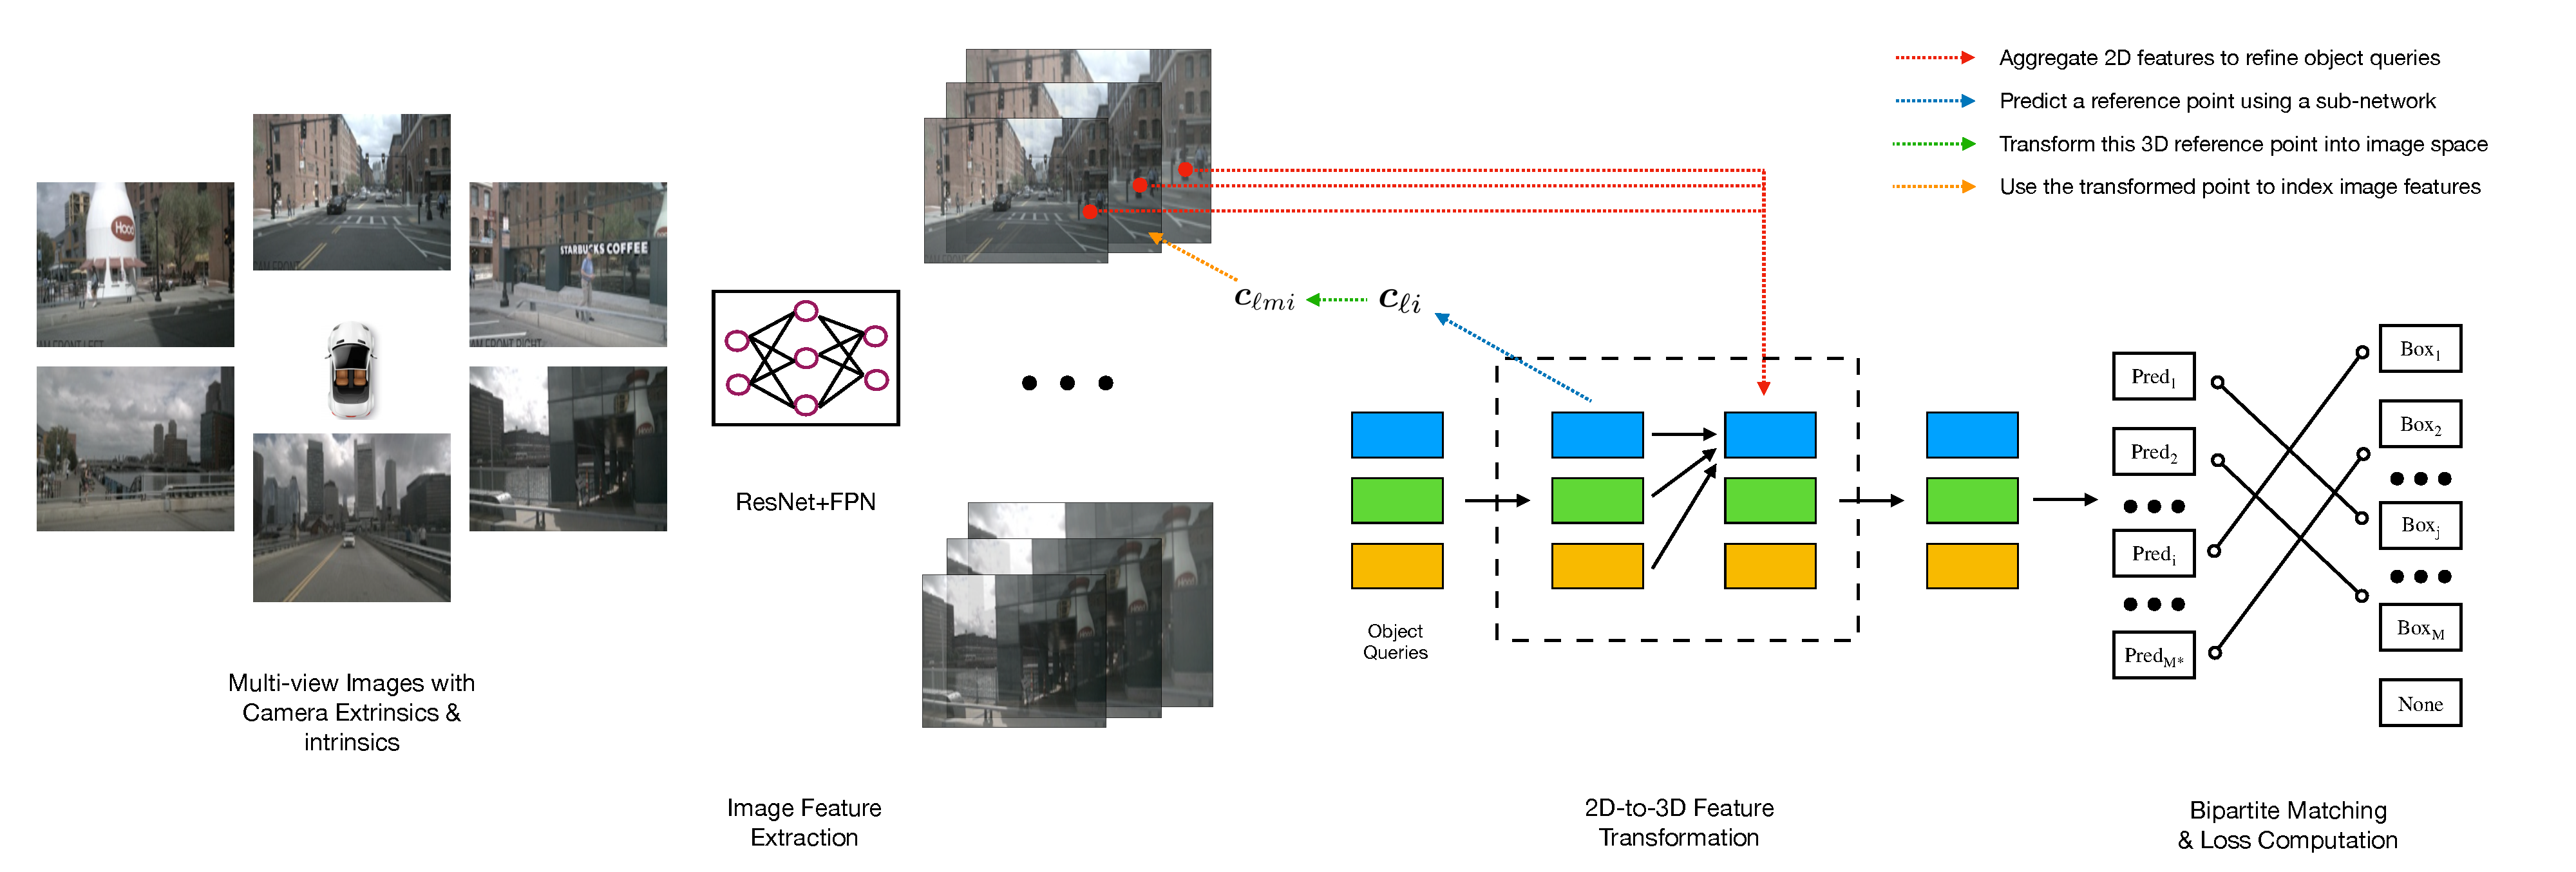
\includegraphics[width=1.0\columnwidth]{figure/architecture}
    \vspace{-1em}
  \caption{本文方法概述。模型输入为一组多视角图像，经ResNet和FPN编码后，模型在一组稀疏的目标查询上操作，每个查询解码为一个3D参考点。通过将3D参考点投影到图像空间，提取2D特征以优化目标查询。模型对每个查询进行预测，并使用集合到集合损失。\label{fig:architecture}}
  \vspace{-2em}
\end{figure}

本文通过一个新的集合预测模块满足这些需求，该模块在2D和3D计算之间交替，连接2D特征提取与3D框预测。模型包含三个关键组件，如图~\ref{fig:architecture}所示。首先，遵循2D视觉中的常见做法，使用共享的ResNet~\cite{He2015}骨干网络从相机图像中提取特征，并可选地使用特征金字塔网络（Feature Pyramid Network, FPN）~\cite{Lin2017}增强这些特征（\S\ref{feature-learning}）。其次，检测头（\S\ref{detection-head}）——本文的主要贡献——以几何感知的方式将计算得到的2D特征与一组3D边界框预测连接起来（\S\ref{detection-head}）。检测头的每一层从一组稀疏的目标查询开始，这些查询从数据中学习得到。每个目标查询编码一个3D位置，该位置被投影到相机平面并通过双线性插值收集图像特征。与DETR~\cite{detr}类似，使用多头注意力~\cite{Vaswani2017}通过融入目标交互来优化目标查询。该层重复多次，在特征采样和目标查询优化之间交替。最后，使用集合到集合损失~\cite{StewartAN16,detr}训练网络（\S\ref{loss}）。

\subsection{特征学习}
\label{feature-learning}
模型以一组图像 $\I=\{\mathrm{\mathbf{im}}_1, \ldots, \mathrm{\mathbf{im}}_K\} \subset\R^{\mathrm{H_{im}}\times \mathrm{W_{im}}\times3}$（由环视相机拍摄）、相机矩阵 $\T=\{T_1, \ldots, T_K\} \subset \R^{3\times4}$、真值边界框 $\B=\{\bb_1, \ldots, \bb_j, \ldots, \bb_M\}\subset\R^9$ 和类别标签 $\C = \{c_1, \ldots, c_j, \ldots, c_M\}\subset\mathbb{Z}$ 为输入。每个 $\bb_j$ 包含在鸟瞰视图（Bird's-Eye View, BEV）中的位置、尺寸、朝向角和速度；本文旨在从图像中预测这些边界框及其标签。本文\emph{不}使用通常由高端激光雷达捕获的点云。

% \justin{fix the 4,  6 constants ``hard coded'' below---move those to experiments and use letters}
这些图像经ResNet~\cite{He2015}和FPN~\cite{Lin2017}编码为四组特征 $\F_1, \F_2, \F_3, \F_4$。每组特征 $\F_k=\{\bff_{k1}, \ldots, \bff_{k6}\} \subset \R^{H\times W \times C}$ 对应6张图像的一个特征层级。这些多尺度特征提供了丰富的信息，以识别不同大小的目标。下面详细阐述如何通过新颖的集合预测模块将这些2D特征转换为3D特征。

% \subsection{Object Queries}
% \label{object-query}

\subsection{检测头}
\label{detection-head}

现有的从相机输入进行目标检测的方法通常采用自底向上的方式，即对每张图像预测一组密集的边界框，在图像间过滤冗余框，并在后处理步骤中聚合所有相机的预测。该范式有两个关键缺陷：密集边界框预测需要准确的深度感知（这本身就是一个具有挑战性的问题）；基于NMS的冗余去除和聚合是不可并行化的操作，会引入显著的推理开销。本文通过下面描述的自顶向下检测头来解决这些问题。

与~\cite{objdgcnn, zhu2021deformable}类似，\name 是\emph{迭代式}的；使用 $L$ 层基于集合的计算从2D特征图中生成边界框估计。每一层包括以下步骤：
\begin{enumerate}
    \item 预测与目标查询关联的一组边界框中心；
    \item 使用相机变换矩阵将这些中心投影到所有特征图中；
    \item 通过双线性插值采样特征并将其融入目标查询；
    \item 使用多头注意力描述目标交互。
\end{enumerate}

受DETR~\cite{detr}启发，每一层 $\ell\in\{0,\ldots,L-1\}$ 对一组\emph{目标查询} $\Q_\ell=\{\bq_{\ell 1}, \ldots, \bq_{\ell M^*}\}\subset\R^{C}$ 进行操作，生成新集合 $\Q_{\ell+1}$。从目标查询 $\bq_{\ell i}$ 解码出参考点 $\bc_{\ell i}\in \R^3$：
\begin{equation}\label{eq:query-point}
    \begin{split}
      \bc_{\ell i}=\Phi^{\mathrm{ref}}(\bq_{\ell i}),
    \end{split}
\end{equation}
其中 $\Phi^{\mathrm{ref}}$ 是一个神经网络。$\bc_{\ell i}$ 可视为第 $i$ 个框中心的一个假设。接下来，获取与 $\bc_{\ell i}$ 对应的图像特征，以优化并预测最终的边界框。然后，使用相机变换矩阵将 $\bc_{\ell i}$（更准确地说，其齐次坐标 $\bc_{\ell i}^*$）投影到每张图像中：
\begin{equation}\label{eq:point-projection}
    \begin{split}
      \bc_{\ell i}^* = \bc_{\ell i} \oplus 1 \qquad\qquad \bc_{\ell m i} = T_m \bc_{\ell i}^*,
    \end{split}
\end{equation}
其中 $\oplus$ 表示拼接操作，$\bc_{\ell m i}$ 是参考点在第 $m$ 个相机上的投影。为消除特征图大小的影响并收集不同层级的特征，将 $\bc_{\ell m i}$ 归一化到 $[-1, 1]$。接下来，通过以下方式收集图像特征：
\begin{equation}\label{eq:bilinear}
    \begin{split}
        \bff_{\ell k m i}  = f^{\mathrm{bilinear}}(\F_{km}, \bc_{\ell m i}),
    \end{split}
\end{equation}
其中 $\bff_{\ell k m i}$ 是第 $\ell$ 层中第 $i$ 个点在第 $m$ 个相机第 $k$ 个特征层级上的特征。

给定参考点不一定在所有相机图像中都可见，因此需要使用启发式方法过滤无效点。为此，定义二值变量 $\sigma_{\ell k m i}$，其取值基于参考点是否投影到图像平面之外。最终特征 $\bff_{\ell i}$ 和下一层的目标查询 $\bq_{(\ell+1) i}$ 由下式给出：
\begin{equation}\label{eq:feature-agg}
    \begin{split}
        \bff_{\ell i}  = \frac{1}{\sum_k\sum_m \sigma_{\ell k m i}+\epsilon}\sum_k \sum_m \bff_{\ell k m i} \sigma_{\ell k m i} \qquad \mathrm{and} \qquad \bq_{(\ell+1)i} = \bff_{\ell i}  + \bq_{\ell i},
    \end{split}
\end{equation}
其中 $\epsilon$ 是一个微小数值，用于避免除零。最后，对每个目标查询 $\bq_{\ell i}$，使用两个神经网络 $\Phi_{\ell}^{\mathrm{reg}}$ 和 $\Phi_{\ell}^{\mathrm{cls}}$ 预测边界框 $\hat{\bb}_{\ell i}$ 及其类别标签 $\hat{c}_{\ell i}$：
\begin{equation}\label{eq:prediction}
    \begin{split}
      \hat{\bb}_{\ell i} = \Phi_{\ell}^{\mathrm{reg}}(\bq_{\ell i})  \qquad \mathrm{and} \qquad   \hat{c}_{\ell i} = \Phi_{\ell}^{\mathrm{cls}}(\bq_{\ell i}).
    \end{split}
\end{equation}
在训练期间，对每一层的预测 $\hat{\B}_\ell =\{\hat{\bb}_{\ell 1}, \ldots, \hat{\bb}_{\ell j}, \ldots, \hat{\bb}_{\ell M^\ast}\}\subset\R^9$ 和 $\hat{\C}_\ell = \{\hat{c}_{\ell 1}, \ldots, \hat{c}_{\ell j}, \ldots, \hat{c}_{\ell M}\}\subset\mathbb{Z}$ 计算损失。推理时，只使用最后一层的输出。
% \justin{Something seems to be missing here.  Do you define how you obtain $\B,\C$ used in the next section.  Make sure every step is clear here.  Also, where do you predict the \emph{number} of boxes in the scene?}

\subsection{损失函数}
\label{loss}

参考~\cite{StewartAN16,detr}，使用集合到集合损失来衡量预测集合 $(\hat{\B}_\ell, \hat{\C}_\ell)$ 与真值集合 $(\B, \C)$ 之间的差异。该损失由两部分组成：类别标签的焦点损失（Focal Loss）~\cite{lin2017focal}和边界框参数的 $L^1$ 损失。为书写方便，省略 $\hat{\B}_\ell$ 和 $\hat{\C}_\ell$ 中的下标 $\ell$。真值框的数量 $M$ 通常小于预测数量 $M^\ast$，因此将真值框集合用 $\varnothing$（无目标）填充到 $M^{\ast}$ 以便于计算。通过二分匹配（Bipartite Matching）问题建立真值与预测之间的对应关系：$\sigma^{\ast} = \argmin_{\sigma \in \mathcal{P}}\sum_{j=1}^M -1_{\{c_j\neq\varnothing\}}\hat{p}_{\sigma(j)}(c_j) + 1_{\{c_j=\varnothing\}}\mathcal{L}_{\mathrm{box}}(\bb_j, \hat{\bb}_{\sigma(j)}),$

其中 $\mathcal{P}$ 表示所有排列的集合，$\hat{p}_{\sigma(j)}(c_j)$ 是索引 $\sigma(j)$ 的预测属于类别 $c_j$ 的概率，$\mathcal{L}_{\mathrm{box}}$ 是边界框参数的 $L_1$ 损失。与~\cite{StewartAN16,detr}一样，使用匈牙利算法~\cite{Kuhn55thehungarian}求解该分配问题，得到集合到集合损失 $\mathcal{L_{\mathrm{sup}}} = \sum_{j=1}^N -\log\hat{p}_{\sigma^{\ast}(j)}(c_j) + 1_{\{c_j=\varnothing\}}\mathcal{L}_{\mathrm{box}}(\bb_j, \hat{\bb}_{\sigma^{\ast}(j)})$.
% \begin{equation}\label{eq:sup_loss}
%      \begin{split}
%       \mathcal{L_{\mathrm{sup}}} = \sum_{j=1}^N -\log\hat{p}_{\sigma^{\ast}(j)}(c_j) + 1_{\{c_j=\varnothing\}}\mathcal{L}_{\mathrm{box}}(\bb_j, \hat{\bb}_{\sigma^{\ast}(j)}).
%      \end{split}
% \end{equation}




\section{实验}
实验结果按以下方式呈现：首先在\S\ref{detail}中详细说明数据集、评估指标和实现细节；然后在\S\ref{sota}中将本文方法与现有工作进行对比；在\S\ref{overlap}中评估不同模型在相机重叠区域的性能；在\S\ref{pseudo}中与前向预测模型进行比较；最后在\S\ref{ablation}中提供额外的分析和消融实验。

\subsection{实现细节}
\label{detail}

\textbf{数据集（Dataset）。} 在nuScenes数据集~\cite{nuscenes2019}上进行测试。nuScenes包含1,000个序列，每个序列长约20秒，采样率为20帧/秒。每个样本包含6个相机图像 \texttt{[front\_left, front, front\_right, back\_left, back, back\_right]}。提供了包括内参和外参在内的相机参数。nuScenes每0.5秒提供一次标注，训练集、验证集和测试集分别有28k、6k和6k个标注样本。从全部23个类别中选取10个类别用于计算评估指标。

\textbf{评估指标（Metrics）。} 遵循nuScenes提供的官方评估协议。评估平均平移误差（Average Translation Error, ATE）、平均尺度误差（Average Scale Error, ASE）、平均朝向误差（Average Orientation Error, AOE）、平均速度误差（Average Velocity Error, AVE）和平均属性误差（Average Attribute Error, AAE）。这些指标是真正例指标（True Positive Metrics, TP Metrics），以物理单位计算。此外，还测量平均精度（mean Average Precision, mAP）。为全面捕获检测任务的所有方面，定义了一个综合标量指标——nuScenes检测得分（nuScenes Detection Score, NDS）~\cite{nuscenes2019}：$\mathrm{NDS} = \frac{1}{10}[5\mathrm{mAP}+\sum_{\mathrm{mTP}\in \mathbb{TP}}(1-\min(1, \mathrm{mTP}))]$。
% \begin{equation}
%     \begin{split}
%     \mathrm{NDS} = \frac{1}{10}[5\mathrm{mAP}+\sum_{\mathrm{mTP}\in \mathbb{TP}}(1-\min(1, \mathrm{mTP}))].
%     \end{split}
% \end{equation}

\textbf{模型（Model）。} 本文模型由ResNet~\cite{He2015}特征提取器、FPN和\name 检测头组成。使用在第3和第4阶段具有可变形卷积~\cite{dai17dcn}的ResNet101。FPN~\cite{Lin2017}接收ResNet输出的特征，生成4张尺寸分别为输入图像大小$\nicefrac18$、$\nicefrac1{16}$、$\nicefrac1{32}$和$\nicefrac1{64}$的特征图。\name 检测头包含6层，每层由一个特征优化步骤和一个多头注意力层组成。\name 检测头的隐藏维度为256。最后，两个子网络分别预测每个目标查询的边界框参数和类别标签；每个子网络由两个隐藏维度为256的全连接层组成。在检测头中使用层归一化（LayerNorm）~\cite{BaKH16}。

\textbf{训练与推理（Training \& Inference）。} 使用AdamW~\cite{loshchilov2018decoupled}训练整个流程。权重衰减为$10^{-4}$。初始学习率为$10^{-4}$，在第8和第11个epoch分别降至$10^{-5}$和$10^{-6}$。模型总共训练12个epoch，使用8张RTX 3090 GPU，每GPU批大小为1。训练过程大约需要18小时。推理时不使用NMS等后处理。评估使用nuScenes评估工具包。

\subsection{与现有工作对比}
\label{sota}
与之前的当前最优方法CenterNet~\cite{zhou2019centernet}和FCOS3D~\cite{wang2021fcos3d}进行比较。CenterNet是一种无锚框2D检测方法，在高分辨率特征图上进行密集预测。FCOS3D采用FCOS~\cite{tian2019fcos}流程进行逐像素预测。这两种方法都将3D目标检测转化为2D问题，因此忽略了场景几何和传感器配置。为执行多视角目标检测，这些方法必须独立处理每张图像，并分别使用逐图像和全局NMS来去除各视角和重叠区域中的冗余框。如表~\ref{table:sota}所示，本文方法即使不使用任何后处理，也优于这些方法。本文方法在mATE指标上略逊于FCOS3D，推测是因为FCOS3D直接预测边界框深度，从而对目标平移提供了强监督。此外，FCOS3D为不同的边界框参数使用了解耦检测头，这有助于提升性能。

在测试集上（表~\ref{table:sota:test}），截至2021年10月13日，本文方法优于所有现有方法；为公平比较，本文方法与DD3D~\cite{dd3d}使用相同的骨干网络。

\begin{table}[t] 
\begin{center}
\caption{在验证集上与近期工作的对比。本文方法对NMS的使用具有鲁棒性。$\ast$：CenterNet使用自定义骨干网络DLA~\cite{Yu_2018_CVPR}。$\ddag$：该模型使用深度权重1.0训练，并从FCOS3D检查点初始化；该检查点在同一数据集上使用深度权重0.2训练。$\S$：使用测试时数据增强。$\P$：使用测试时数据增强、更多epoch和模型集成。详见\cite{wang2021fcos3d}。$\dag$：本文方法同样从FCOS3D骨干网络初始化；检测头随机初始化。$\#$：使用CBGS~\cite{cbgs}训练。\label{table:sota}}
\vspace{-1.0em}
\resizebox{\linewidth}{!}{
\begin{tabular}{c|c|c|c|c|c|c|c|c}
\toprule
\hline
方法 & NDS $\uparrow$ & mAP $\uparrow$ & mATE $\downarrow$ & mASE $\downarrow$ & mAOE $\downarrow$ & mAVE $\downarrow$ & mAAE $\downarrow$ & NMS \\
\hline
CenterNet  $\ast$ & 0.328 & 0.306 & 0.716 & 0.264 & 0.609 & 1.426 & 0.658 & \checkmark \\
\hline
FCOS3D  & 0.373 & 0.299 & 0.785 & 0.268 & 0.557 & 1.396 & 0.154 & \checkmark \\
\hline
\changed{FCOS3D $\ddag$} & \changed{0.393} & \changed{0.321} & \changed{0.746} & \changed{0.265} & \changed{0.503} & \changed{1.351} & \changed{0.160} & \changed{\checkmark} \\

\hline

\changed{FCOS3D $\S$} & \changed{0.402} & \changed{0.326} & \changed{0.743} & \changed{0.259} & \changed{0.441} & \changed{1.341} & \changed{0.163} & \changed{\checkmark} \\

\hline

\changed{FCOS3D $\P$} & \changed{0.415} & \changed{0.343} & \changed{0.725} & \changed{0.263} & \changed{0.422} & \changed{1.292} & \changed{0.153} & \changed{\checkmark} \\

\hline

\name (Ours)   &  0.374 & 0.303 & 0.860 & 0.278 & 0.437 & 0.967 & 0.235 & - \\
\hline
\changed{\name (Ours) $\dag$} & \changed{0.425} & \changed{0.346} & \changed{0.773} & \changed{0.268} & \changed{0.383} & \changed{0.842} & \changed{0.216} & \changed{-} \\
\hline

\changed{\name (Ours) $\#$} & 0.434 & 0.349 & 0.716 & 0.268 & 0.379 & 0.842 & 0.200 & - \\
\hline

\bottomrule
\end{tabular}
}
\end{center}
\end{table}


\begin{table}[t] 
\begin{center}
\caption{在测试集上与排行榜上最优方法的对比。\label{table:sota:test} $\#$：从DD3D检查点初始化。$\dag$：从额外数据预训练的骨干网络初始化。}
\vspace{-0.5em}
\resizebox{\linewidth}{!}{
\begin{tabular}{c|c|c|c|c|c|c|c|c}
\toprule
\hline
方法 & NDS $\uparrow$ & mAP $\uparrow$ & mATE $\downarrow$ & mASE $\downarrow$ & mAOE $\downarrow$ & mAVE $\downarrow$ & mAAE $\downarrow$ & NMS \\
\hline 
Mono3D & 0.429 & 0.366 & 0.642 & 0.252 & 0.523 & 1.591 & 0.119 & N/A \\ 
\hline 
DHNet & 0.437 & 0.363 & 0.667 & 0.259 & 0.402 & 1.589 & 0.120 & N/A \\ 
\hline 
PGD~\cite{wang2021probabilistic} & 0.448 & 0.386 & 0.626 & 0.245 & 0.451 & 1.509 & 0.127 & \checkmark \\ 
\hline
DD3D~\cite{dd3d} $\dag$ & 0.477 & 0.418 & 0.572 & 0.249 & 0.368 & 1.014 & 0.124 & \checkmark \\
\hline
\name (Ours) $\#$ & 0.479 & 0.412 & 0.641 & 0.255 & 0.394 & 0.845 & 0.133 & - \\
\hline
\bottomrule
\end{tabular}
}
\end{center}
\end{table}


\subsection{重叠区域对比}
\label{overlap}
重叠区域是一个巨大挑战，因为目标更容易被截断。本文方法同时考虑所有相机，而FCOS3D则逐相机独立预测边界框。为进一步展示融合推理的优势，计算落入相机重叠区域的边界框的评估指标。具体而言，选择3D中心被多个相机可见的框。在验证集上，共有18,147个这样的框，占总数的9.7%。表~\ref{table:overlap}展示了结果；在该设置下，本文方法在NDS得分上显著优于FCOS3D。这证实了集成预测方法更加有效。

\begin{table}[t] 
\begin{center}
% \vspace{-1.0em}
\caption{重叠区域对比。$\ddag$：该模型使用深度权重1.0训练，并从FCOS3D检查点初始化；该检查点在同一数据集上使用深度权重0.2训练。详见\cite{wang2021fcos3d}。$\dag$：本文方法同样从FCOS3D骨干网络初始化；检测头随机初始化。\label{table:overlap}}
% \vspace{-1.0em}
\resizebox{\linewidth}{!}{
\begin{tabular}{c|c|c|c|c|c|c|c|c}
\toprule
\hline
方法 & NDS $\uparrow$ & mAP $\uparrow$ & mATE $\downarrow$ & mASE $\downarrow$ & mAOE $\downarrow$ & mAVE $\downarrow$ & mAAE $\downarrow$ & NMS \\
\hline
\hline
FCOS3D & 0.317 & 0.213 & 0.841 & 0.276 & 0.604 & 1.122 & 0.173 &  \checkmark \\
\hline
\changed{FCOS3D}$\ddag$ & \changed{0.329} & \changed{0.229} & \changed{0.816} & \changed{0.272} & \changed{0.571} & \changed{1.084} & \changed{0.195} &  \changed{\checkmark} \\
\hline
\name (Ours)  &  0.356 & 0.231 & 0.825 & 0.280 & 0.400 & 0.863 & 0.223 & - \\
\hline
\changed{\name (Ours)} $\dag$ &  \changed{0.384} & \changed{0.268} & \changed{0.807} & \changed{0.273} & \changed{0.453} & \changed{0.788} & \changed{0.184} & \changed{-} \\
\hline
\bottomrule
\end{tabular}
}
\end{center}
% \vspace{-2.5em}
\end{table}


\subsection{与伪激光雷达方法对比}
\label{pseudo}
另一种执行3D目标检测的方式是使用深度预测模型从多视角图像生成伪激光雷达点云。在nuScenes数据集上，没有公开可用的伪激光雷达工作可供直接比较。因此，自行实现一个基线方法以验证本文方法优于显式深度预测。使用预训练的PackNet~\cite{packnet}网络从所有六个相机预测密集深度图，然后使用相机变换将这些深度图转换为点云。还尝试了带有速度监督的自监督PackNet模型（如原始论文所述），但发现真值深度监督能生成更真实的点云，因此使用有监督模型作为基线。对于3D检测，采用最近提出的CenterPoint架构~\cite{yin2021center}。从概念上讲，该流程是伪激光雷达（Pseudo-LiDAR）~\cite{wang2019pseudo}的一个变体。表~\ref{pseudolidar}展示了结果；即使深度估计由当前最优模型生成，该伪激光雷达方法仍显著不如本文方法。一个可能的解释是，伪激光雷达目标检测器受到不准确深度预测引入的累积误差的影响，而深度预测本身容易过拟合训练数据且对其他数据分布泛化能力差~\cite{demistifying}。%, while our approach does not use depth at all.%<--- debatable  
% \vitor{Are there any published Pseudo-LiDAR methods that we can also use as comparison? It would make this part more convincing, right now feels like we just came up with something to compare and outperformed it, there is no weight to that}

\begin{table}[t] 
\begin{center}
\caption{与伪激光雷达方法对比。\label{pseudolidar}}
\vspace{-1em}
\resizebox{\linewidth}{!}{
\begin{tabular}{c|c|c|c|c|c|c|c|c}
\toprule
\hline
方法 & NDS $\uparrow$ & mAP $\uparrow$ & mATE $\downarrow$ & mASE $\downarrow$ & mAOE $\downarrow$ & mAVE $\downarrow$ & mAAE $\downarrow$ & NMS \\
\hline
pseudo-LiDAR & 0.160 & 0.048 & - & - & - & - & - & \checkmark \\
\hline
\name (Ours)  &  0.374 & 0.303 & 0.860 & 0.278 & 0.437 & 0.967 & 0.235 & - \\
\hline
\bottomrule
\end{tabular}
}
\end{center}
  \vspace{-0.8em}
\end{table}

\subsection{消融实验与分析}
\label{ablation}

图~\ref{fig:iter-refine}可视化了目标查询的优化过程。可视化了每一层从目标查询解码出的边界框。随着模型层数加深，预测边界框逐渐逼近真值。左侧子图展示了从所有数据中学习到的共享目标查询先验。表~\ref{tab:ablation}提供了定量结果，表明迭代优化确实显著提升了性能。这表明迭代优化对于充分利用本文提出的架构既有益又必要。此外，表~\ref{tab:queries}提供了目标查询数量的消融实验；增加查询数量持续提升性能，直到在900个查询时饱和。最后，表~\ref{tab:backbone}展示了不同骨干网络的结果。

\begin{table}[t] 
\begin{center}
  \vspace{-0.8em}
\caption{不同层检测结果的评估。\label{tab:ablation}}
%   \vspace{-0.8em}
\resizebox{0.8\linewidth}{!}{
\begin{tabular}{c|c|c|c|c|c|c|c}
\toprule
\hline
层数 $\uparrow$ & NDS $\uparrow$ & mAP $\uparrow$ & mATE $\downarrow$ & mASE $\downarrow$ & mAOE $\downarrow$ & mAVE $\downarrow$ & mAAE $\downarrow$  \\
\hline
0 & \changed{0.380} & \changed{0.302}  & \changed{0.855} & \changed{0.280} & \changed{0.435} & \changed{0.910} & \changed{0.231}  \\
\hline
1  &  \changed{0.410} & \changed{0.335} & \changed{0.791} & \changed{0.275} & \changed{0.408} & \changed{0.887} & \changed{0.217} \\
\hline
2  & \changed{0.420} & \changed{0.343} & \changed{0.782} & \changed{0.271} & \changed{0.395} & \changed{0.851} & \changed{0.214} \\
\hline
3  & \changed{0.420} & \changed{0.346} & \changed{0.778} & \changed{0.268} & \changed{0.390} & \changed{0.874} & \changed{0.218} \\
\hline
4  &  \changed{0.424} & \changed{0.346} & \changed{0.777} & \changed{0.268} & \changed{0.389} & \changed{0.855} & \changed{0.217} \\
\hline
5  &  \changed{0.425} & \changed{0.346} & \changed{0.773} & \changed{0.268} & \changed{0.383} & \changed{0.842} & \changed{0.216} \\
\hline
\bottomrule
\end{tabular}
}
\end{center}
  \vspace{-0.8em}
\end{table}

\begin{figure}[t!]  
  \vspace{-0.8em}
    \centering
    \begin{tabular}{@{}ccc@{}}
        第1层 & 第2层 & 第3层 \\
        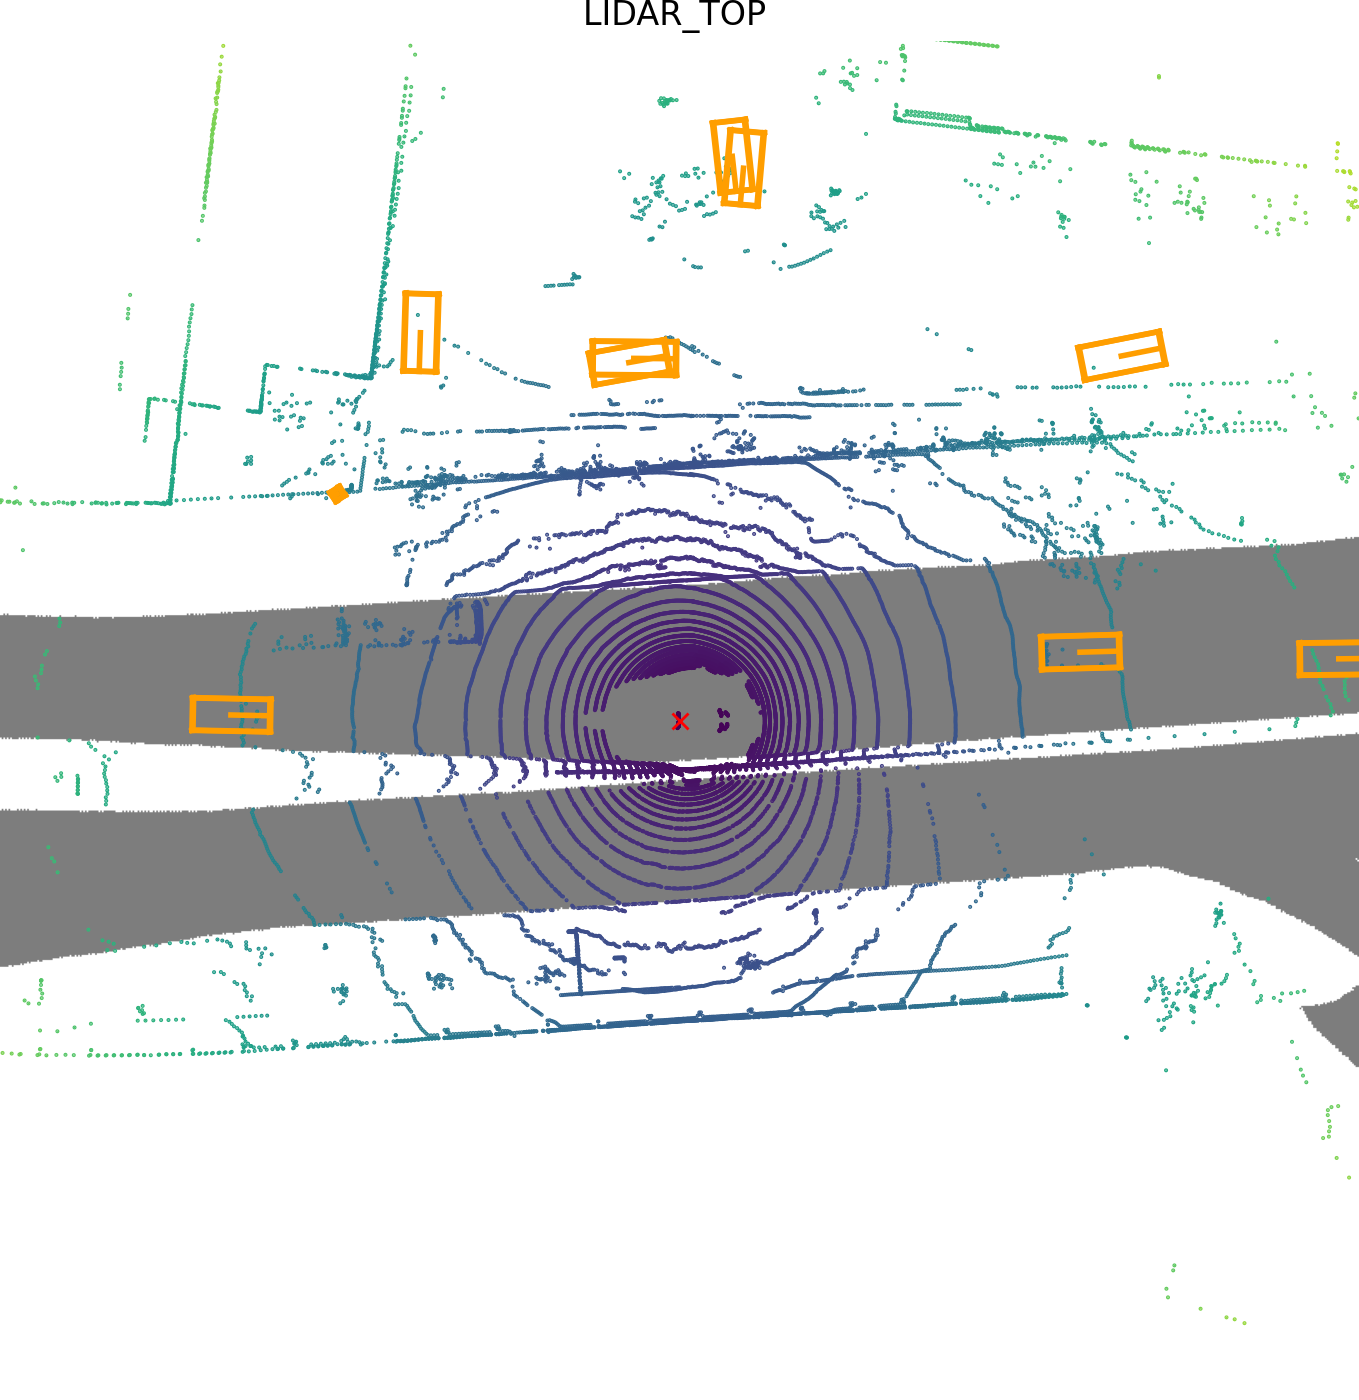
\includegraphics[width=0.31\columnwidth]{figure/iterative_refine_bev/level0.png} & 
    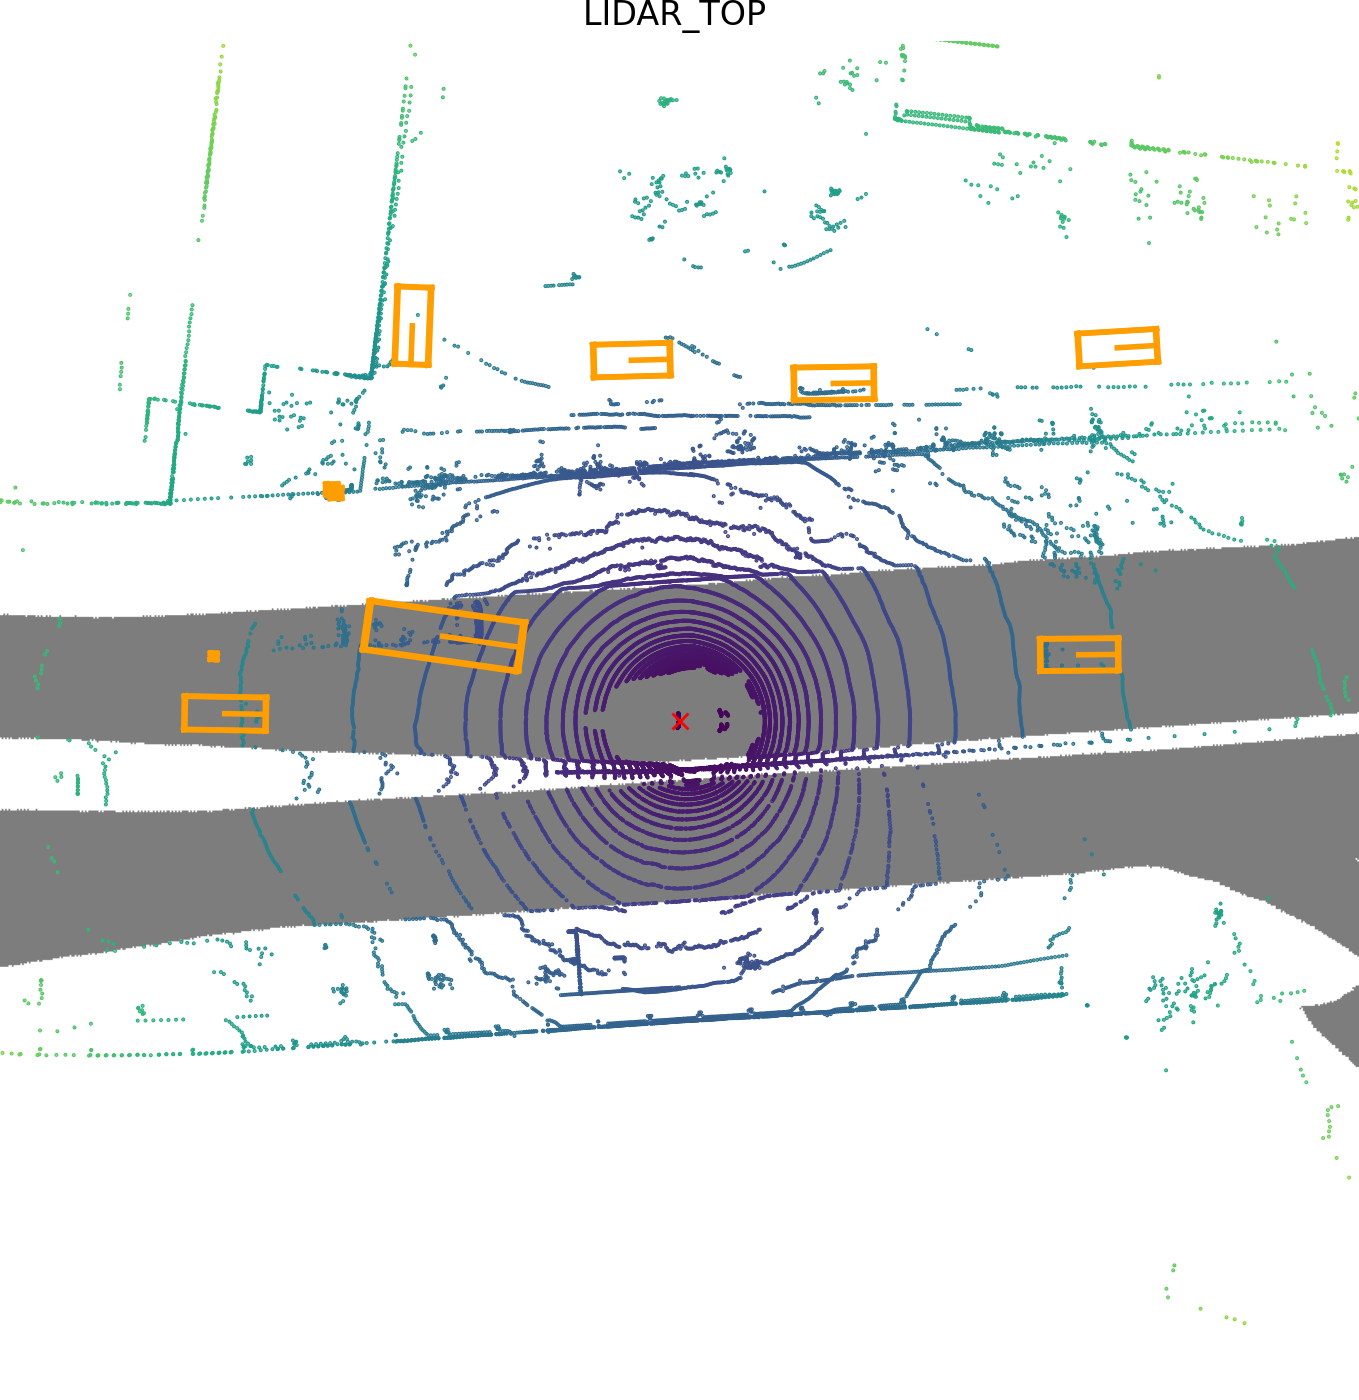
\includegraphics[width=0.31\columnwidth]{figure/iterative_refine_bev/level1.png} &
    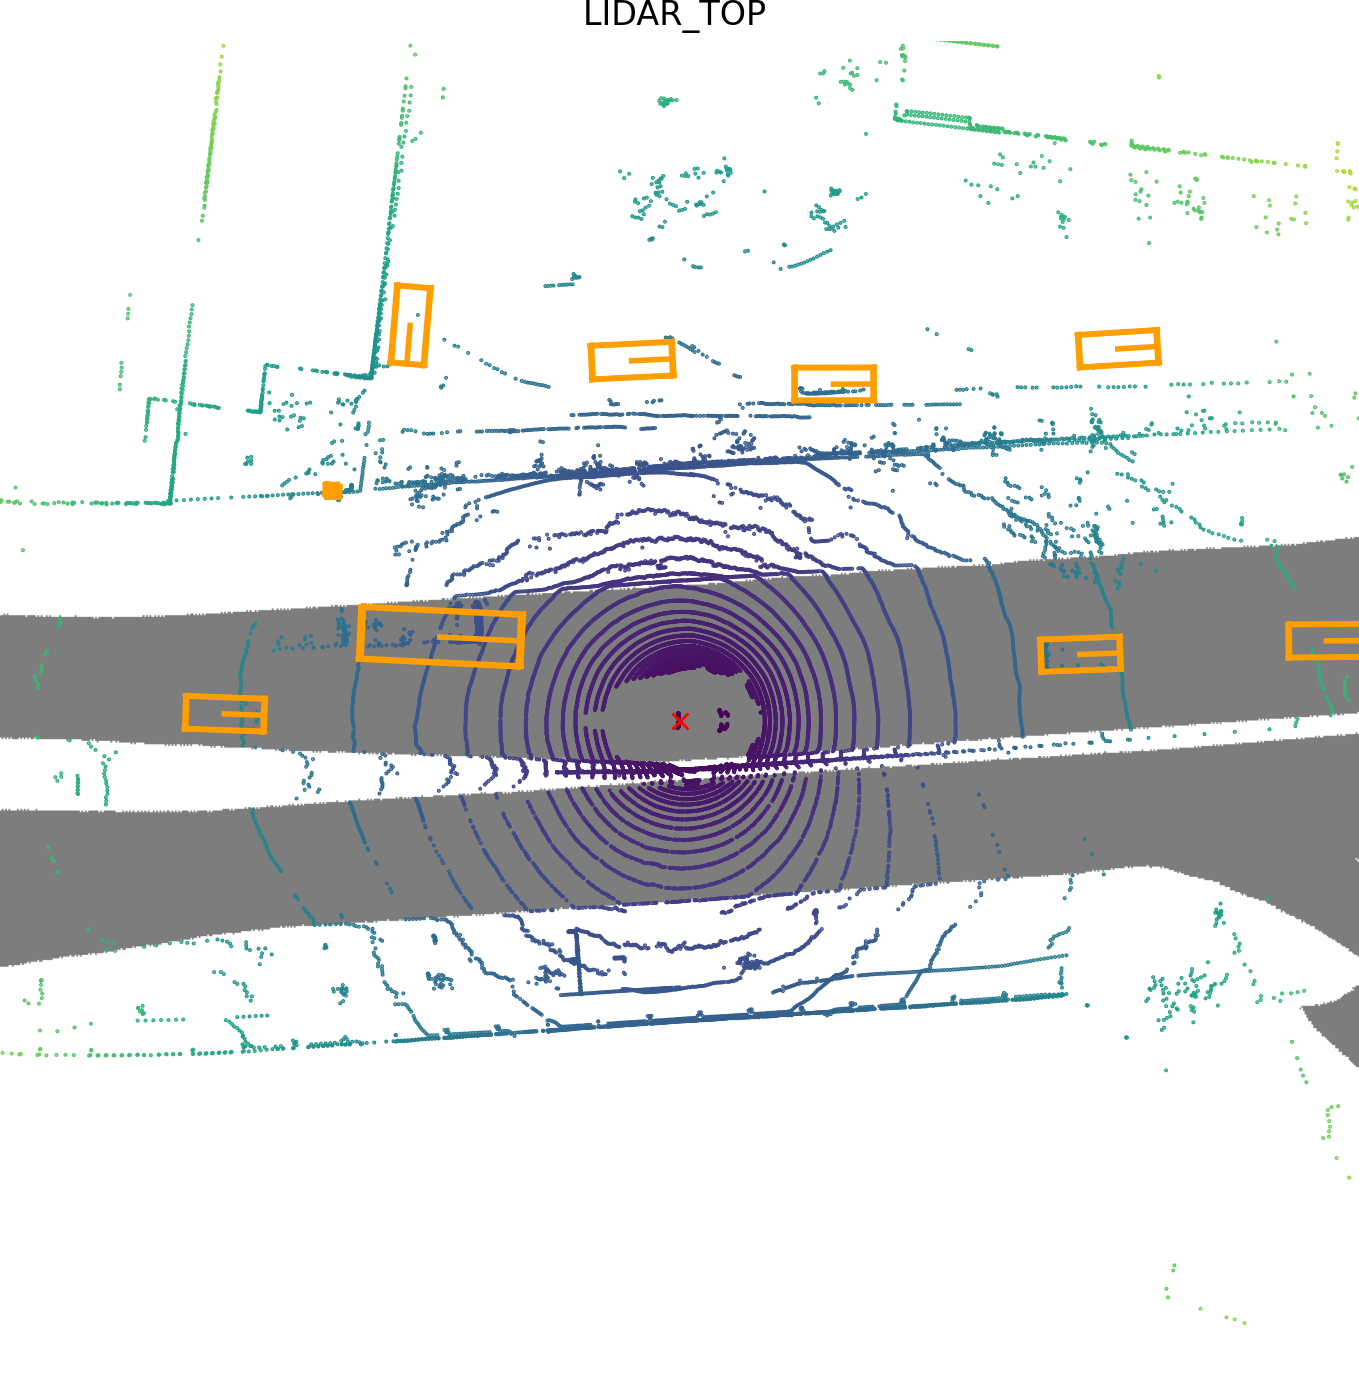
\includegraphics[width=0.31\columnwidth]{figure/iterative_refine_bev/level2.png} \\
        第4层 & 第5层 & 真值 \\
    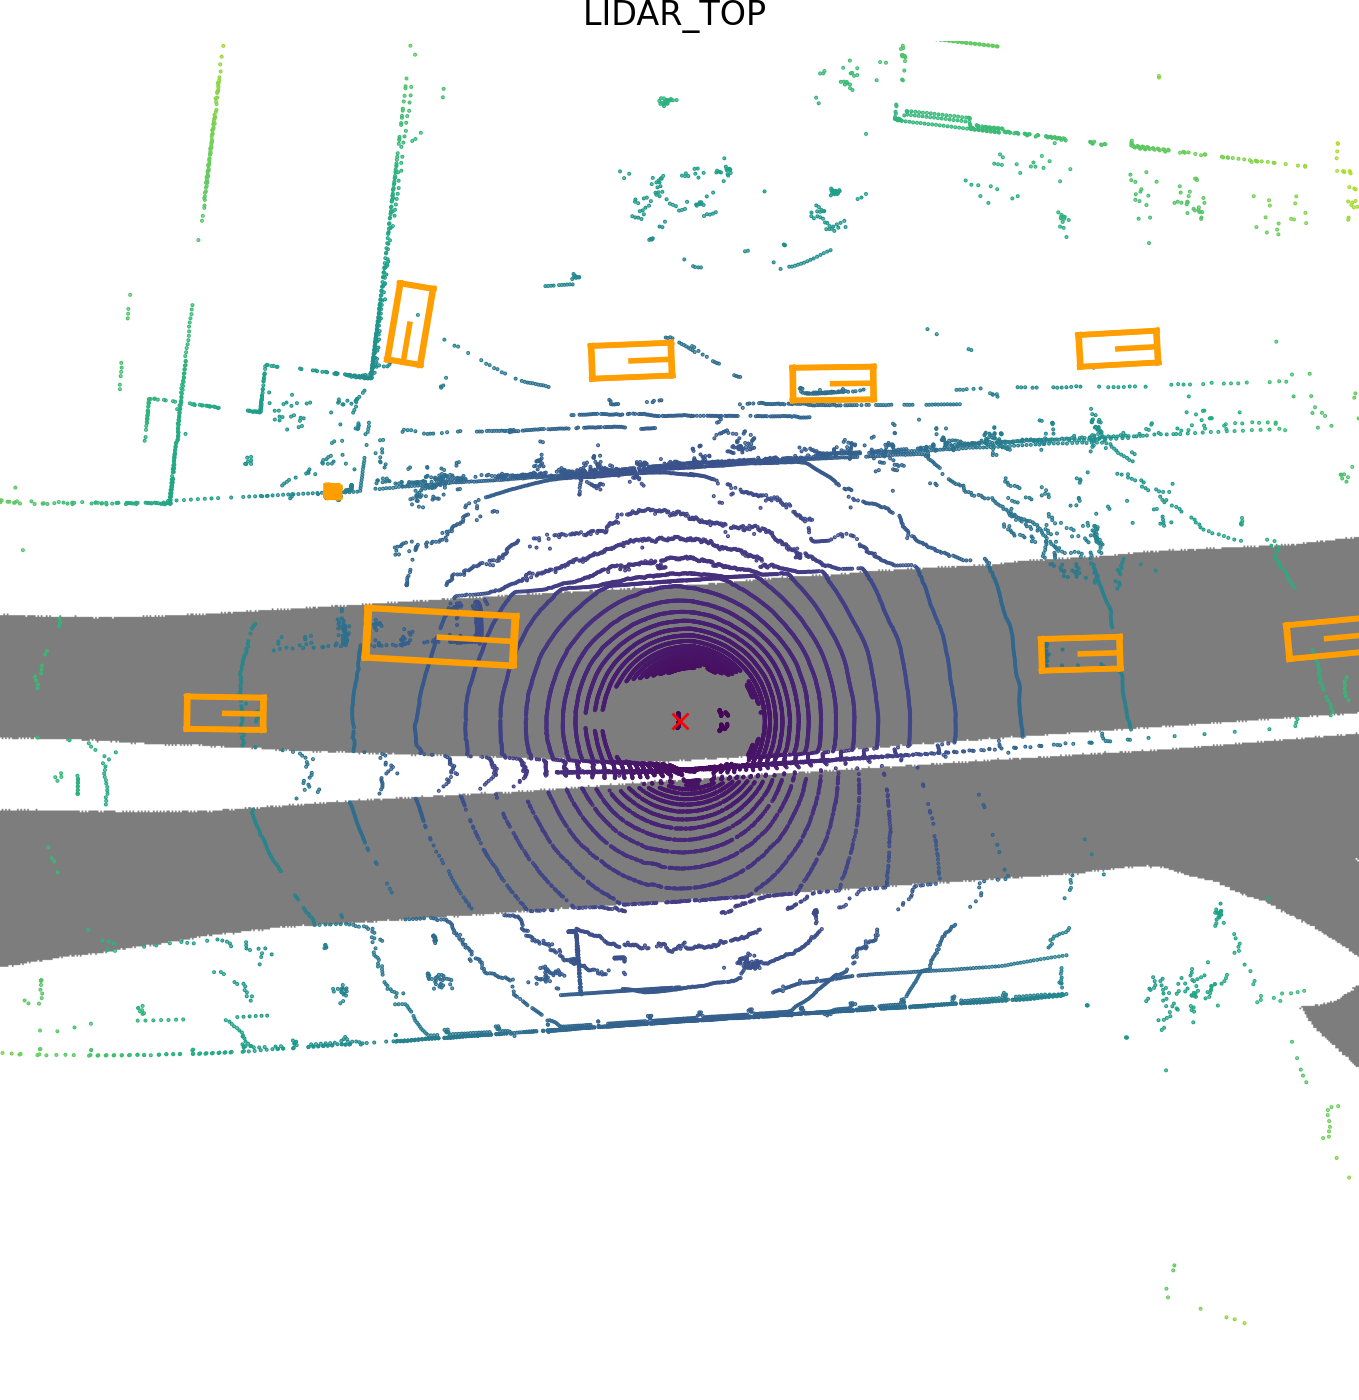
\includegraphics[width=0.31\columnwidth]{figure/iterative_refine_bev/level3.png} & 
    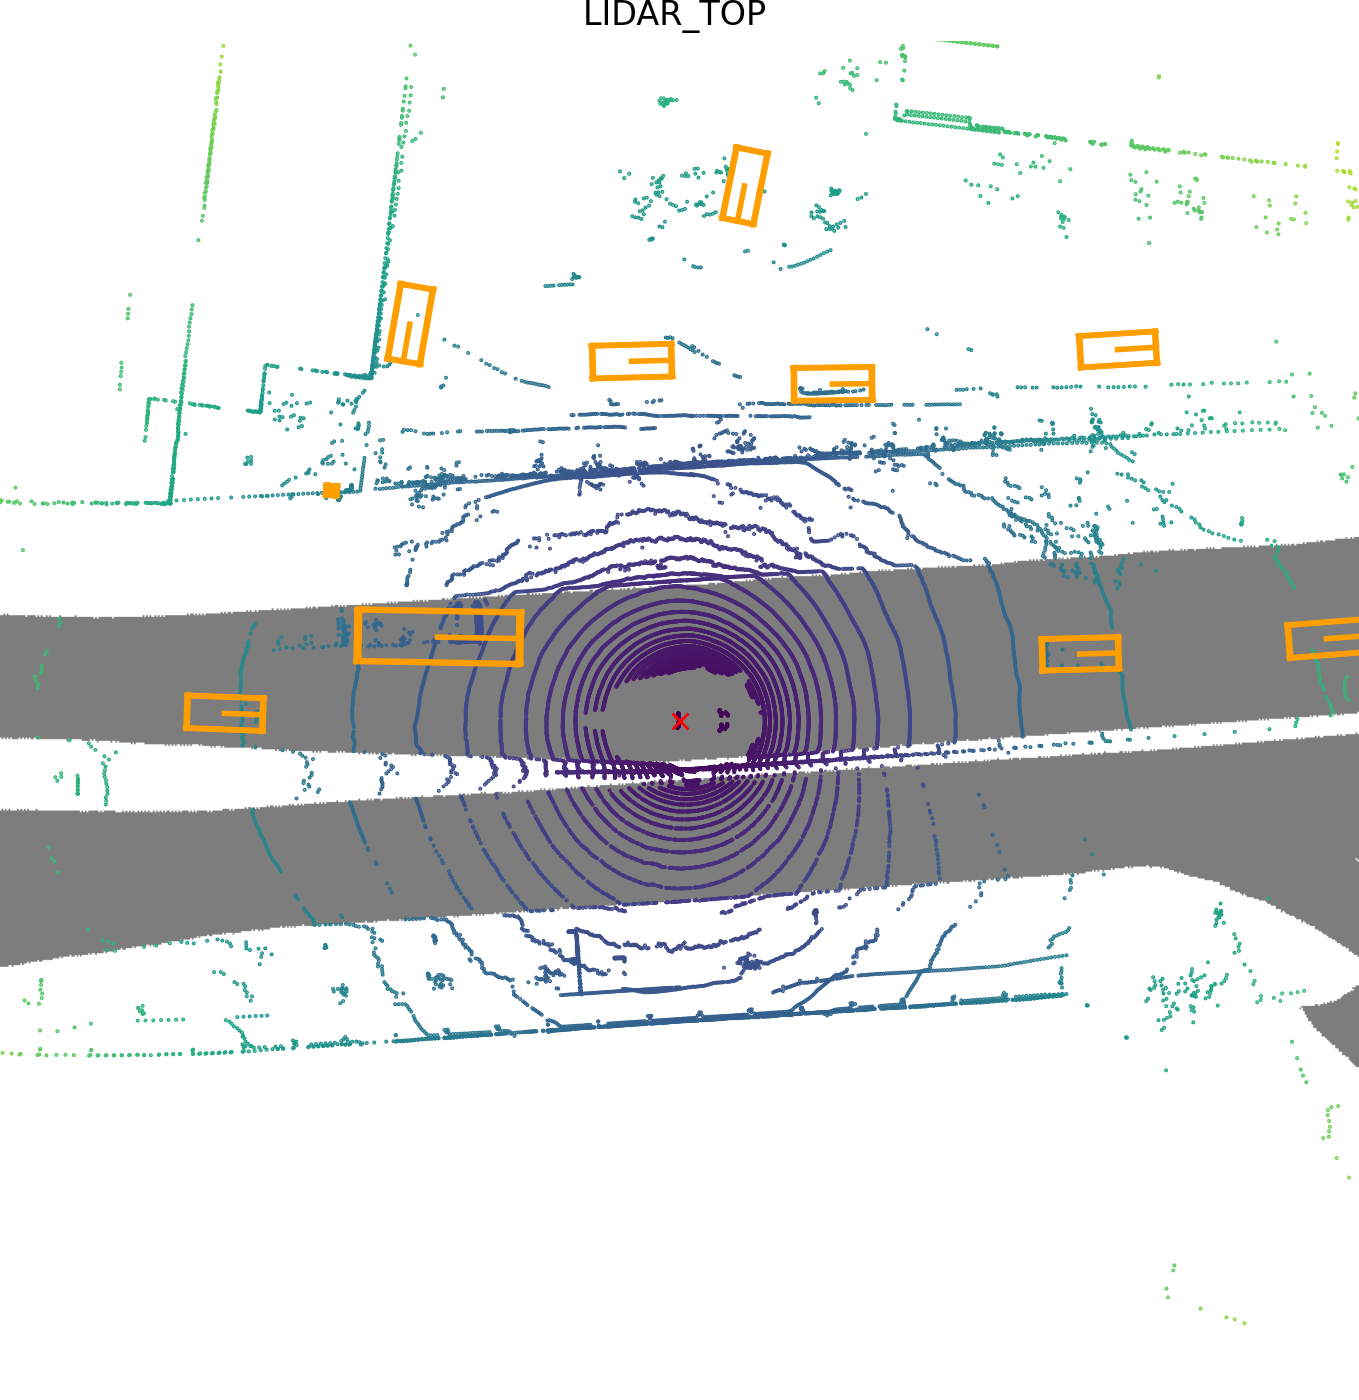
\includegraphics[width=0.31\columnwidth]{figure/iterative_refine_bev/level4.png} & 
        \includegraphics[width=0.31\columnwidth]{figure/iterative_refine_bev/GT-LIDAR_TOP.png} 
    \end{tabular}
%   \vspace{-2.5em}
  \caption{\name 头中第1层到第5层的检测结果。在BEV中可视化边界框，并叠加来自\texttt{lidar\_top}的点云。随着层数加深，预测逐渐接近真值。\label{fig:iter-refine}}
%   \vspace{-2em}
\end{figure}

\begin{table}[t] 
\begin{center}
%   \vspace{-0.8em}
\caption{不同查询数量的结果。\label{tab:queries}}
\resizebox{0.8\linewidth}{!}{
\begin{tabular}{c|c|c|c|c|c|c|c}
\toprule
\hline
\changed{查询数量} & \changed{30} & \changed{100} & \changed{300} & \changed{600} & \changed{900} & \changed{1200} & \changed{1500}  \\
\hline
\changed{mAP $\uparrow$} & \changed{0.201} & \changed{0.313} & \changed{0.338} & \changed{0.347} & \changed{0.346} & \changed{0.340} & \changed{0.346}  \\
\hline
\changed{NDS $\uparrow$} & \changed{0.331} & \changed{0.408} & \changed{0.415} & \changed{0.420} & \changed{0.425} & \changed{0.415} & \changed{0.420}  \\
\bottomrule
\end{tabular}
}
\end{center}
\end{table}

\begin{table}[ht] 
\begin{center}
  \vspace{-1em}
\caption{不同骨干网络的结果。\label{tab:backbone}}
\resizebox{0.8\linewidth}{!}{
\begin{tabular}{c|c|c|c|c|c|c|c}
\toprule
\hline
\changed{骨干网络 $\uparrow$} & \changed{NDS $\uparrow$} & \changed{mAP $\uparrow$} & \changed{mATE $\downarrow$} & \changed{mASE $\downarrow$} & \changed{mAOE $\downarrow$} & \changed{mAVE $\downarrow$} & \changed{mAAE $\downarrow$}  \\
\hline
\changed{ResNet50} & \changed{0.373} & \changed{0.302} & \changed{0.811} & \changed{0.282} & \changed{0.493} & \changed{0.979} & \changed{0.212}  \\
\hline
\changed{ResNet101} & \changed{0.425} & \changed{0.346} & \changed{0.773} & \changed{0.268} & \changed{0.383} & \changed{0.842} & \changed{0.216}\\
\hline
\changed{DLA34} & \changed{0.394} & \changed{0.312} & \changed{0.829} & \changed{0.276} & \changed{0.450} & \changed{0.844} & \changed{0.221} \\
\hline
\bottomrule
\end{tabular}
}
\end{center}
  \vspace{-1em}

\end{table}

图~\ref{fig:prediction}还提供了定性结果，以便直观理解模型性能。将预测的边界框投影到6个相机视图以及BEV视角中。总体而言，本文方法生成了合理的结果，甚至能检测到相对较小的目标。然而，本文方法仍然存在显著的平移误差（与表~\ref{sota}的结果一致）：尽管模型避免了显式深度预测，深度估计仍然是该问题的核心挑战。

% \begin{comment}
\begin{figure}[t!]  
\renewcommand{\arraystretch}{2}

    \centering
    \begin{tabular}{@{}cc@{}}
    \begin{minipage}{.27\textwidth}
        \begin{tabular}{@{}p{1em}@{}c@{}}
        \rotatebox{90}{\small{预测}} & 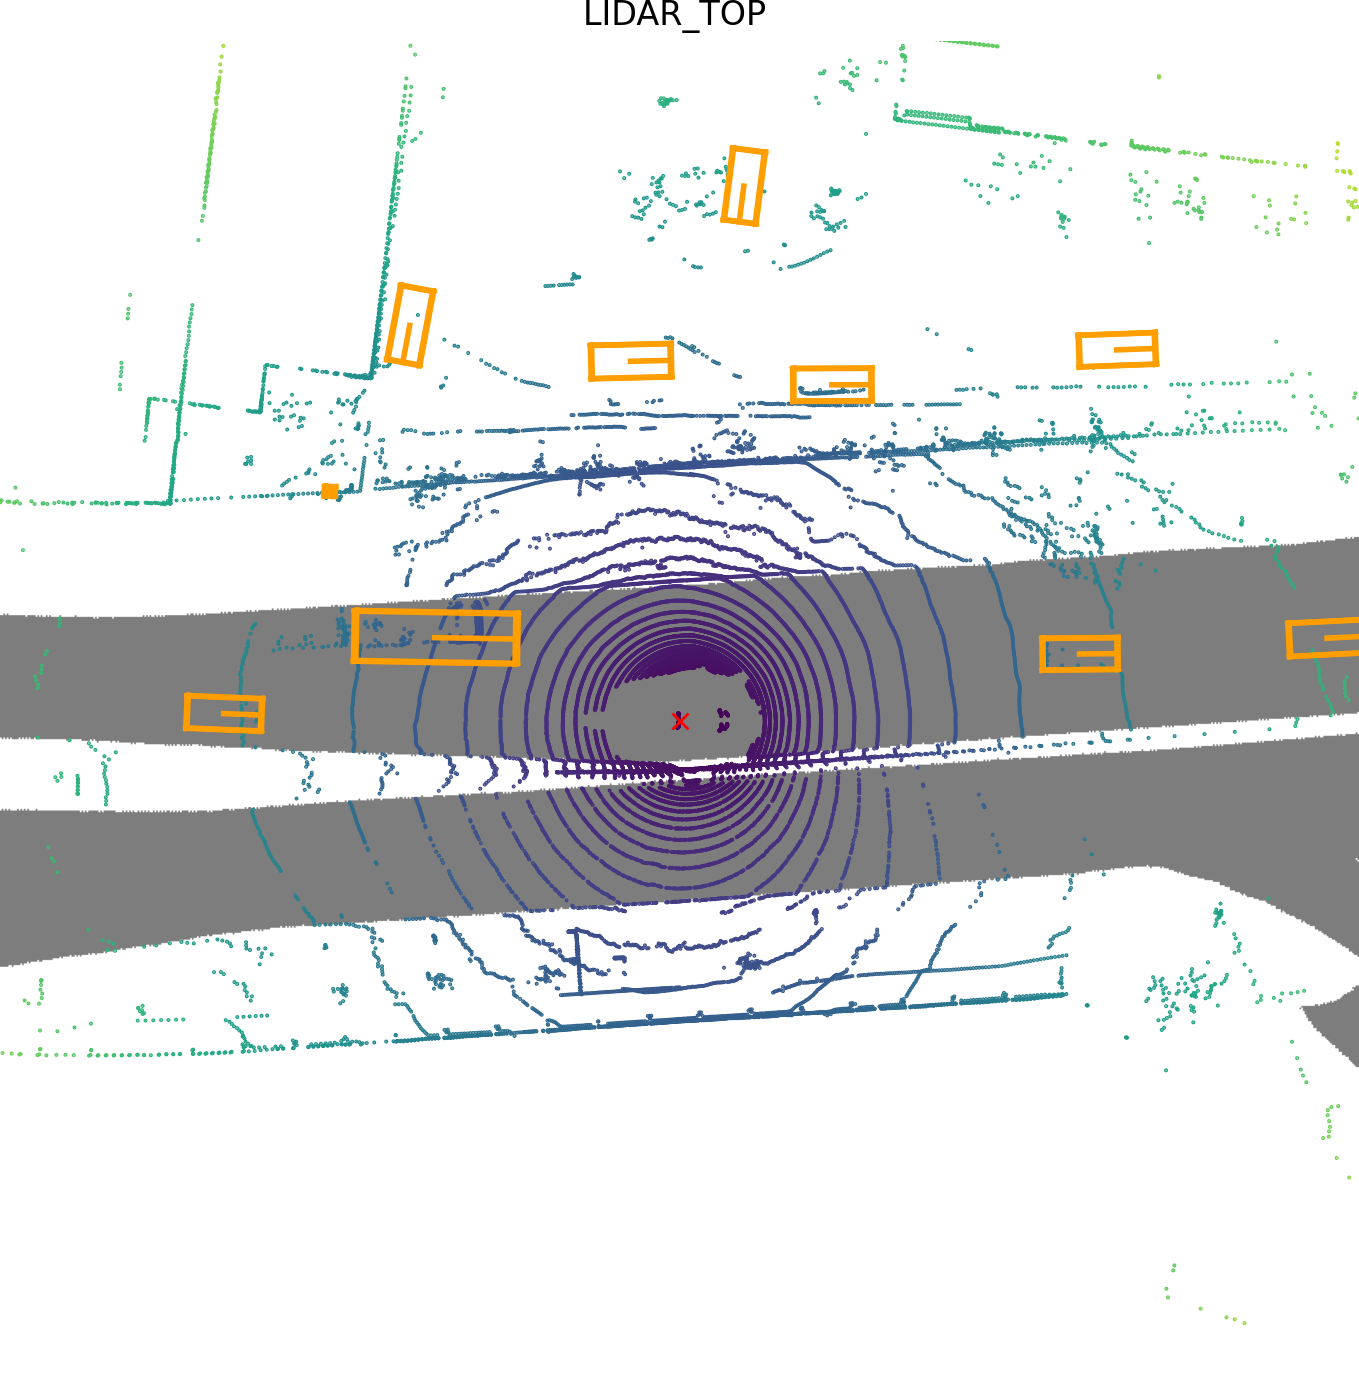
\includegraphics[width=1.0\textwidth]{figure/visualize_predictions/LIDAR_TOP.png}
    \end{tabular}
    \end{minipage}
    & 
    \begin{minipage}{.73\textwidth}
        \begin{tabular}{@{}p{1em}@{}c@{}c@{}c@{}}
        \centering \rotatebox{90}{\small{预测}} &
    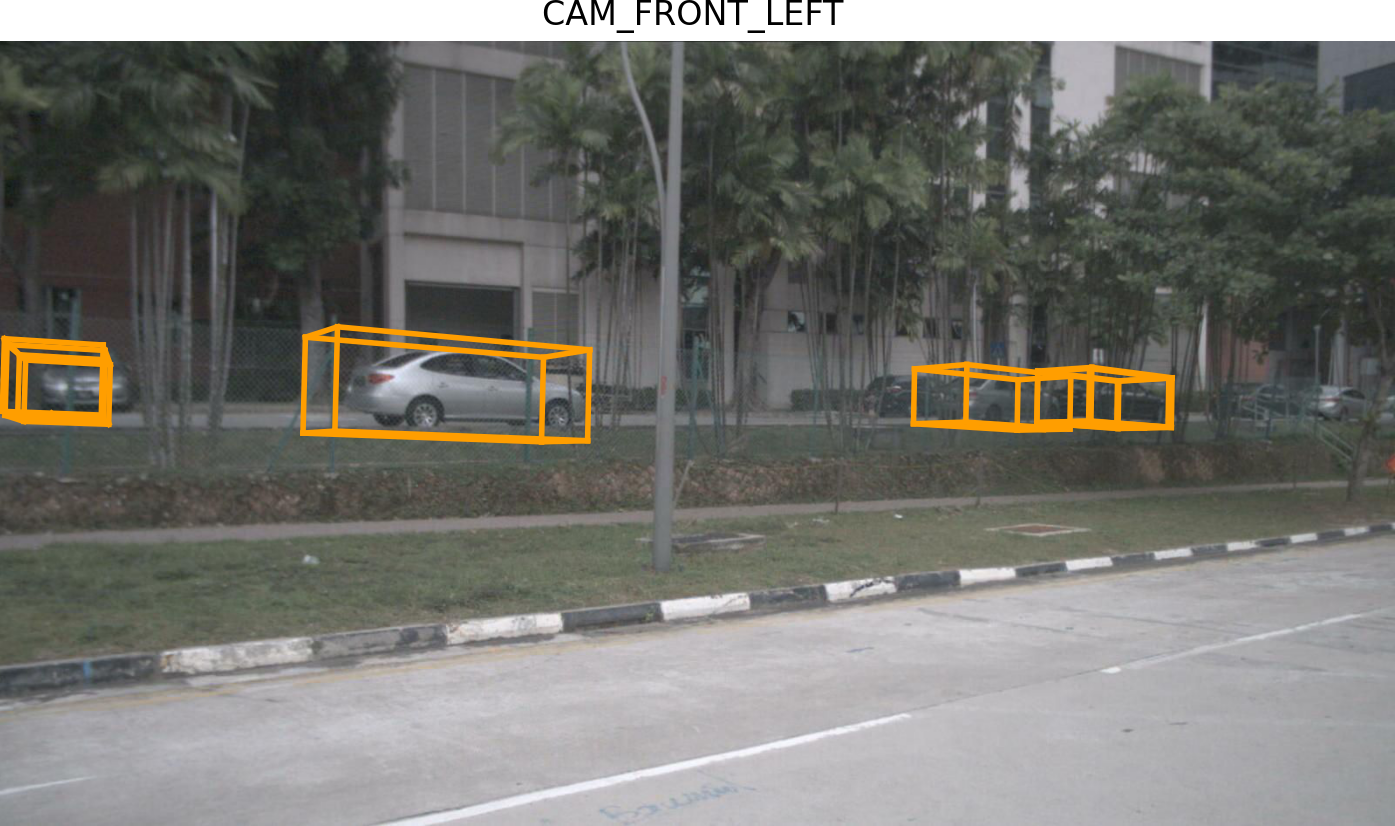
\includegraphics[width=0.31\columnwidth]{figure/visualize_predictions/CAM_FRONT_LEFT.png} & 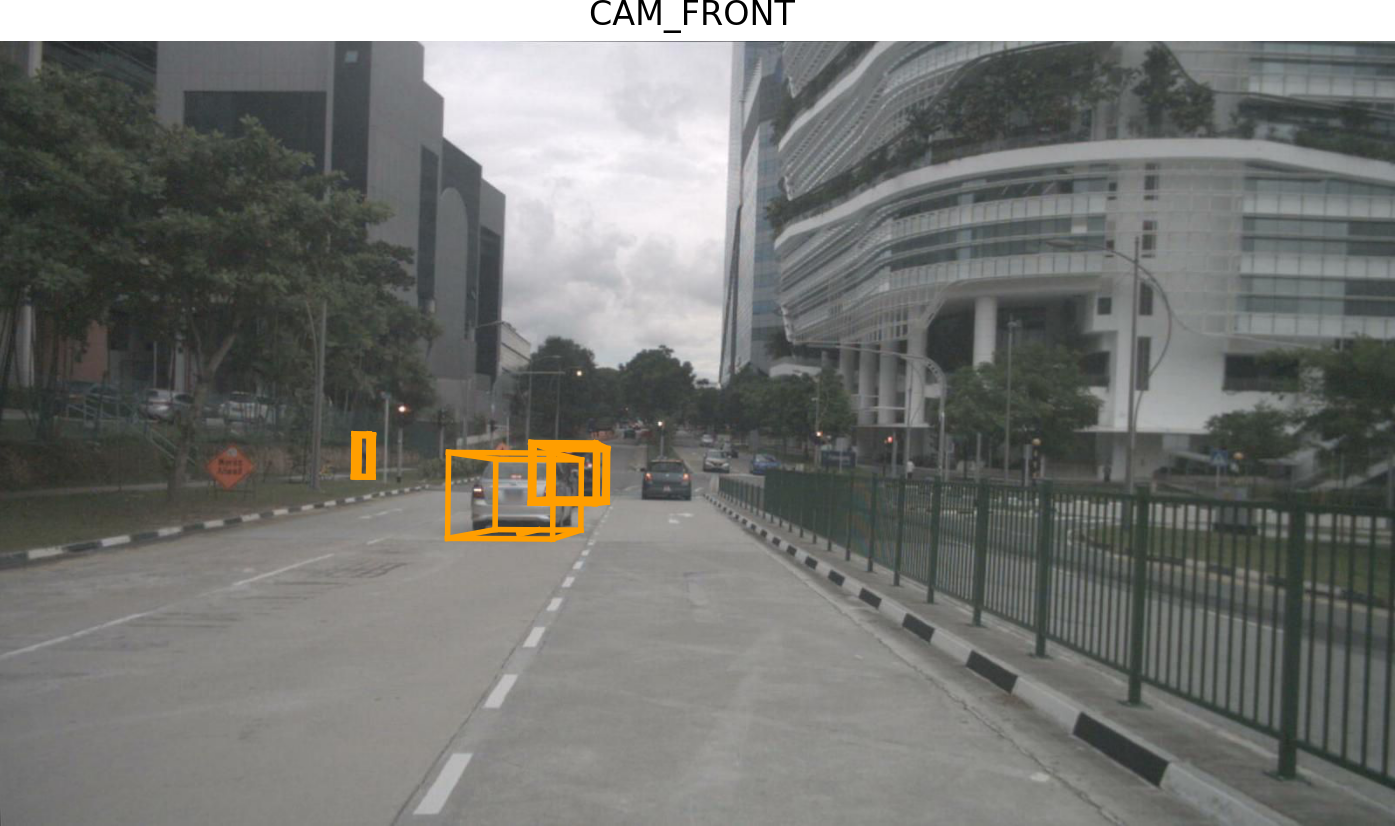
\includegraphics[width=0.31\columnwidth]{figure/visualize_predictions/CAM_FRONT.png} & 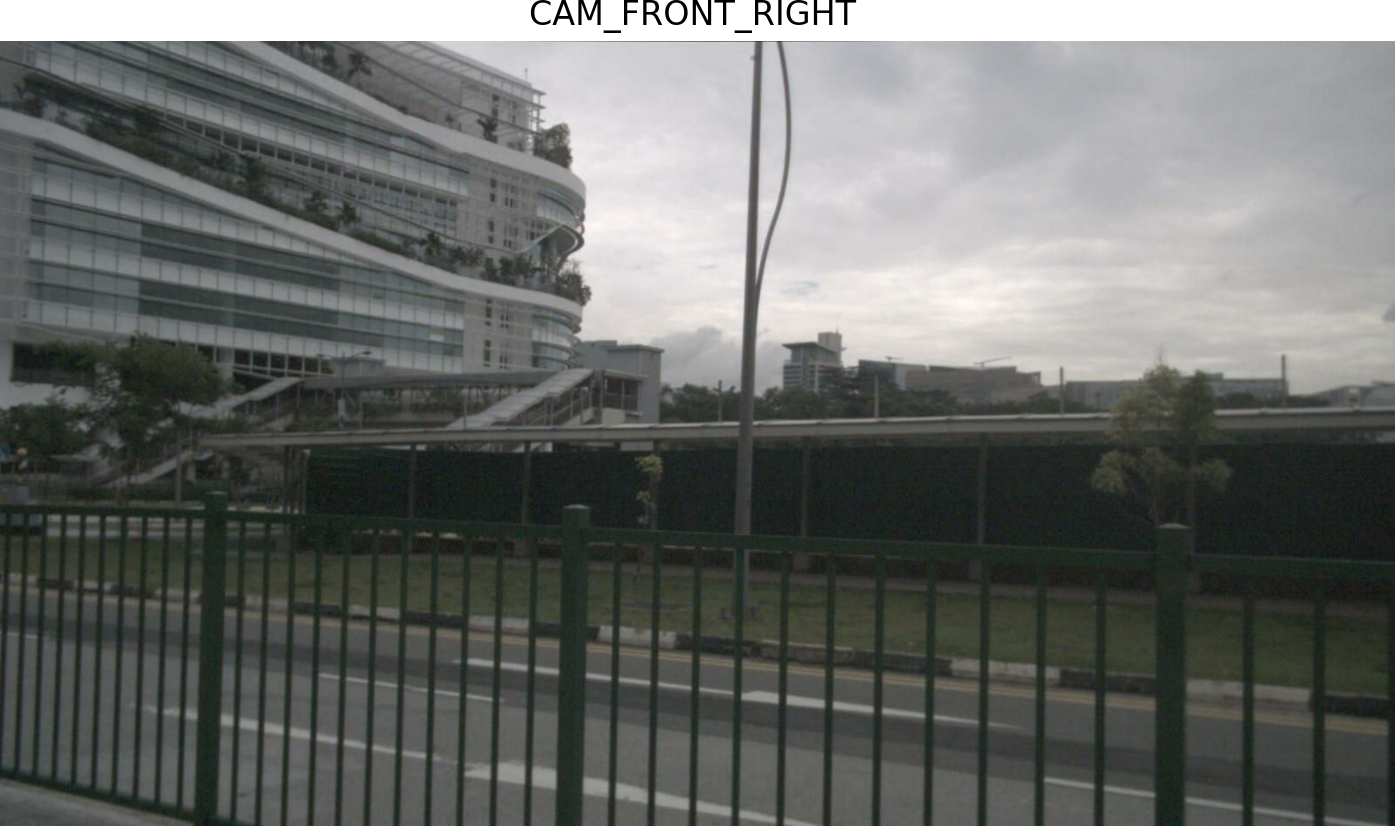
\includegraphics[width=0.31\columnwidth]{figure/visualize_predictions/CAM_FRONT_RIGHT.png} \\ 
            \rotatebox{90}{\small{真值}} &
    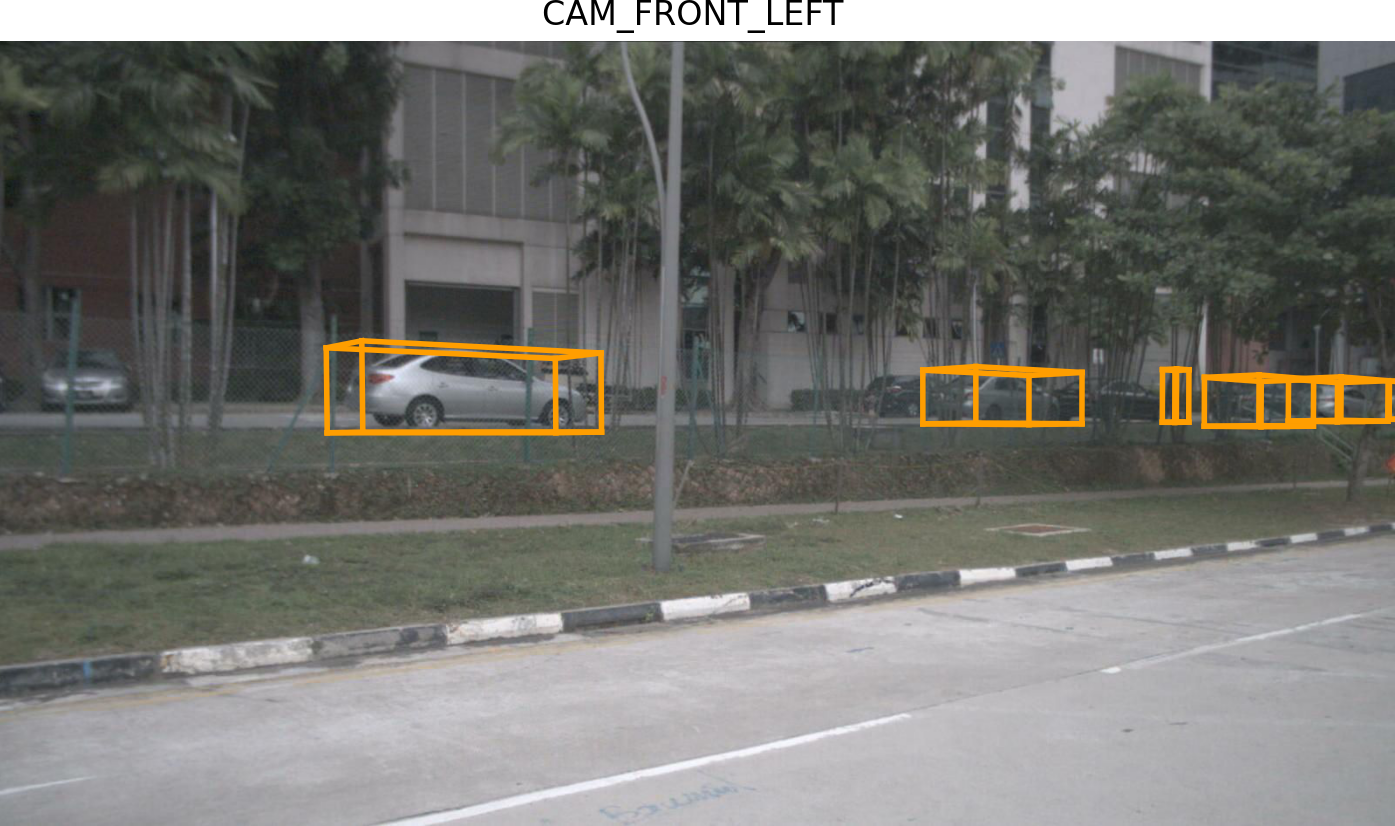
\includegraphics[width=0.31\columnwidth]{figure/visualize_predictions/GT-CAM_FRONT_LEFT.png} & 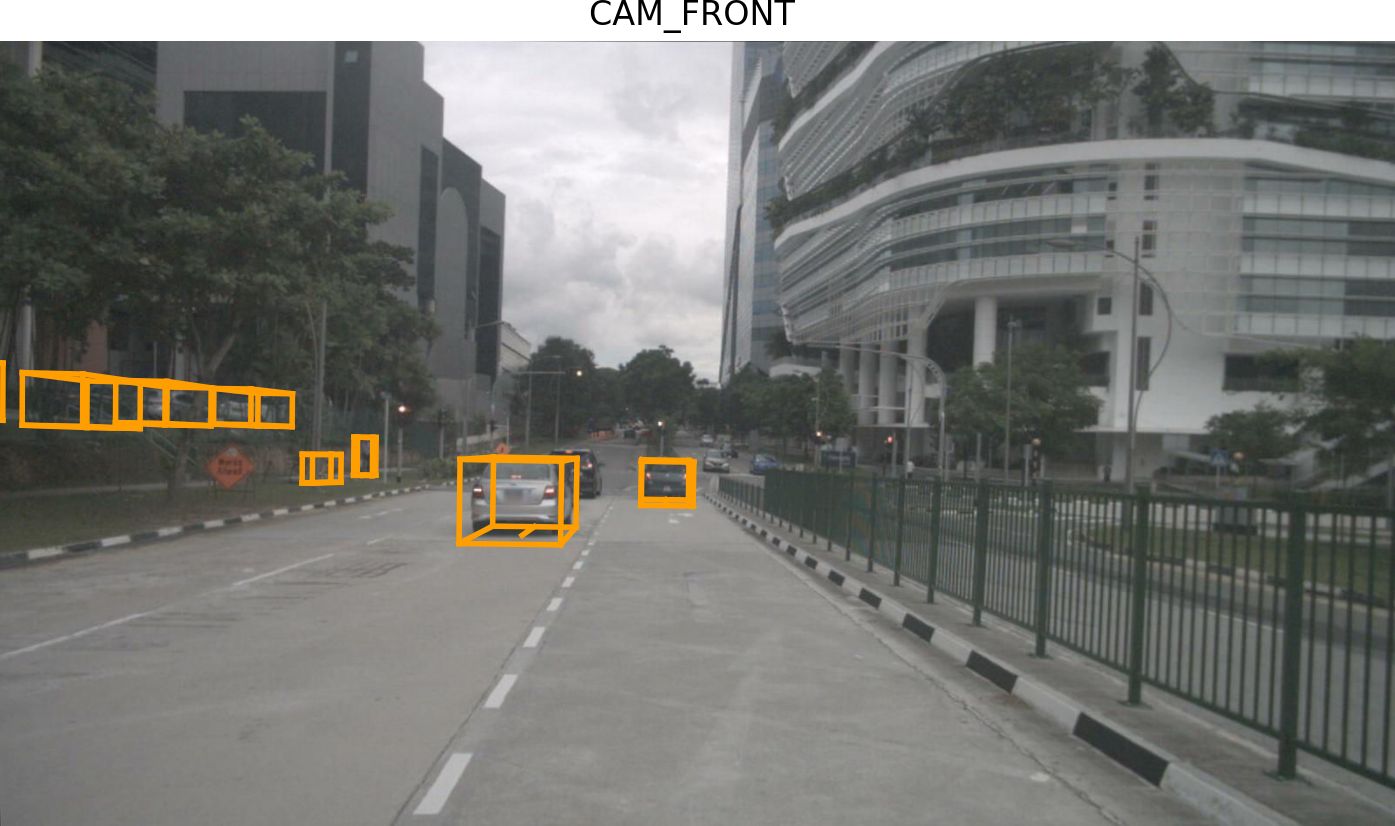
\includegraphics[width=0.31\columnwidth]{figure/visualize_predictions/GT-CAM_FRONT.png} & 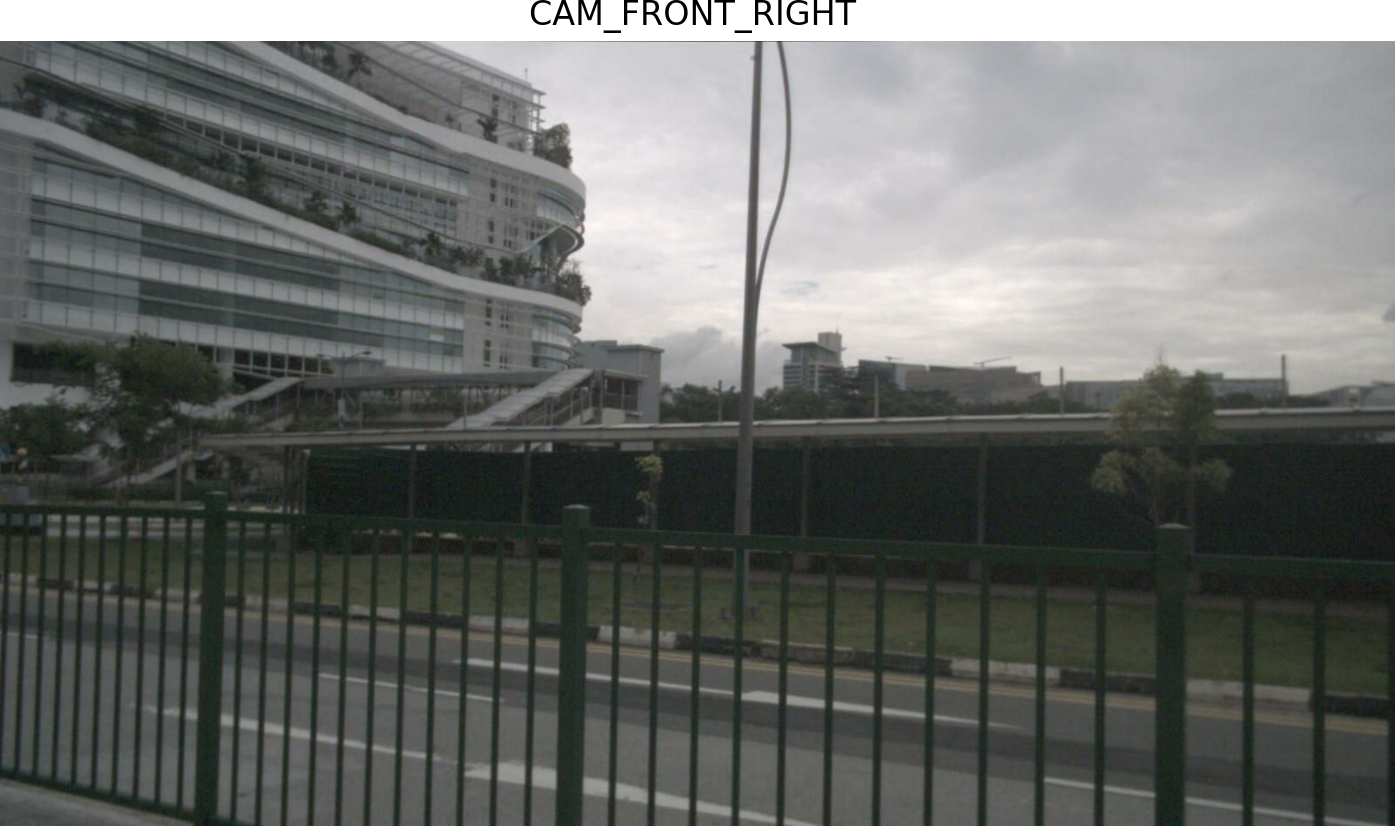
\includegraphics[width=0.31\columnwidth]{figure/visualize_predictions/GT-CAM_FRONT_RIGHT.png} \\ 
    \end{tabular}
    \end{minipage} \\
    
    \begin{minipage}{.27\textwidth}
        \begin{tabular}{@{}p{1em}@{}c@{}}
        \rotatebox{90}{\small{真值}} & \includegraphics[width=1.0\textwidth]{figure/visualize_predictions/GT-LIDAR_TOP.png}
    \end{tabular}
    \end{minipage}
    & 
    \begin{minipage}{.73\textwidth}
        \begin{tabular}{@{}p{1em}@{}c@{}c@{}c@{}}
        \rotatebox{90}{\small{预测}} &
    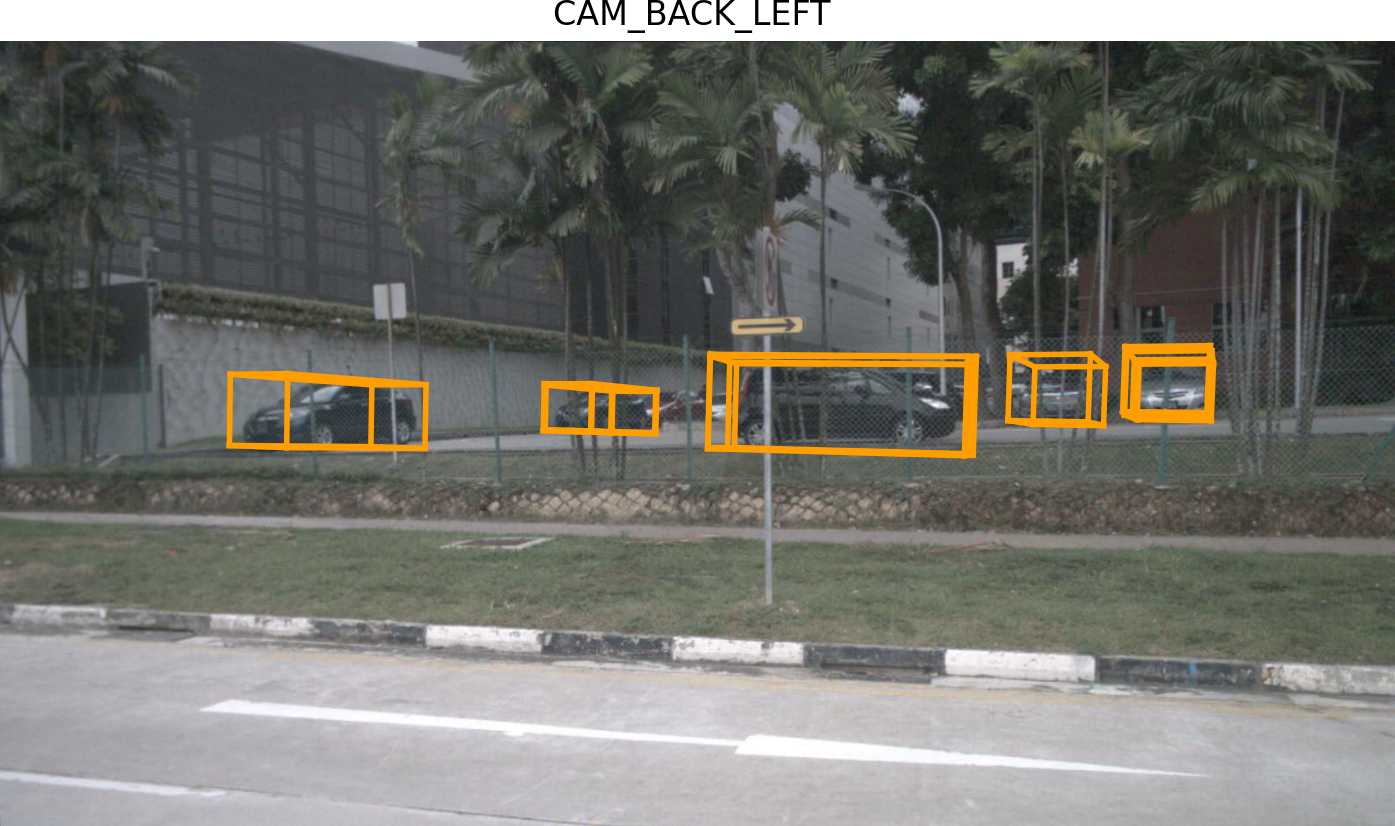
\includegraphics[width=0.31\columnwidth]{figure/visualize_predictions/CAM_BACK_LEFT.png} & 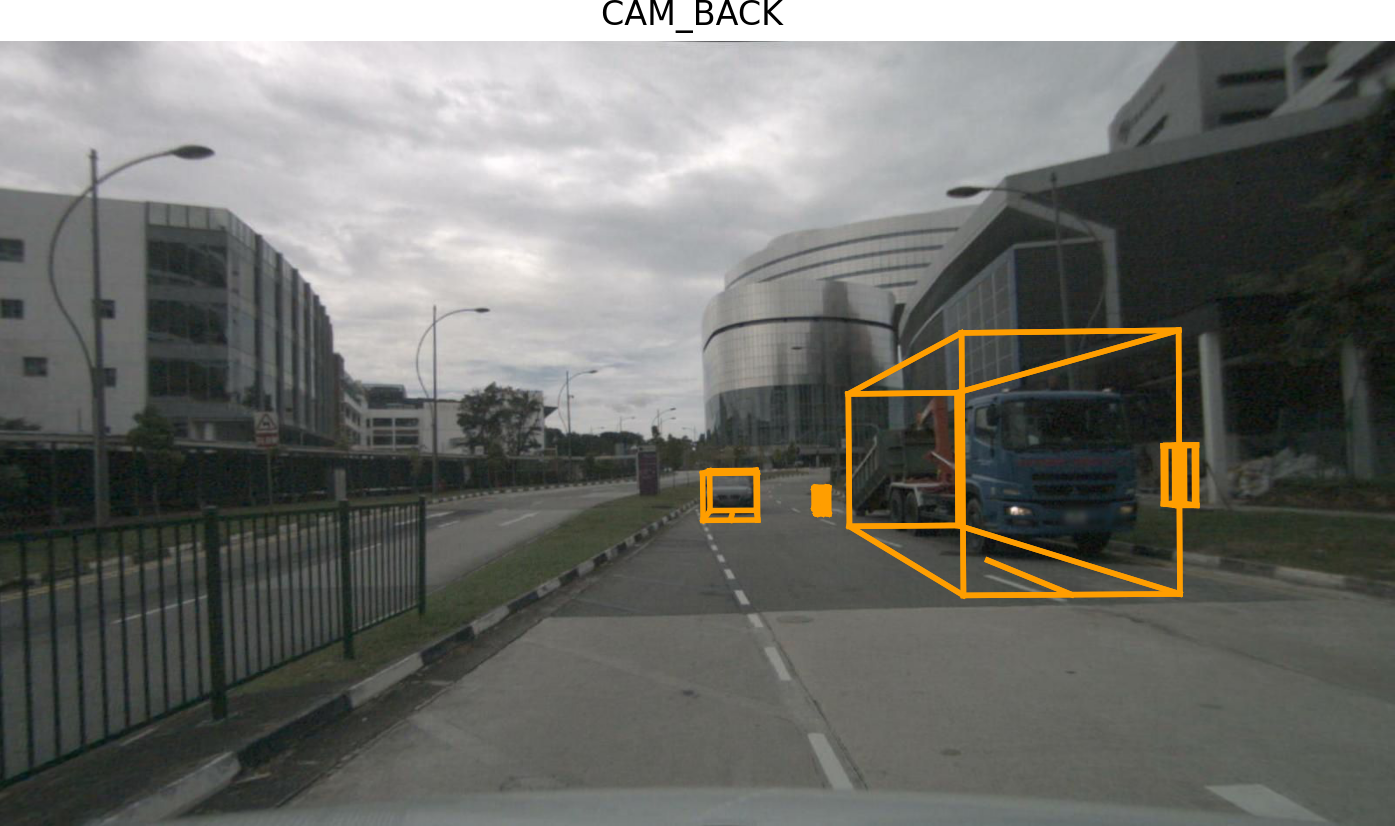
\includegraphics[width=0.31\columnwidth]{figure/visualize_predictions/CAM_BACK.png} & 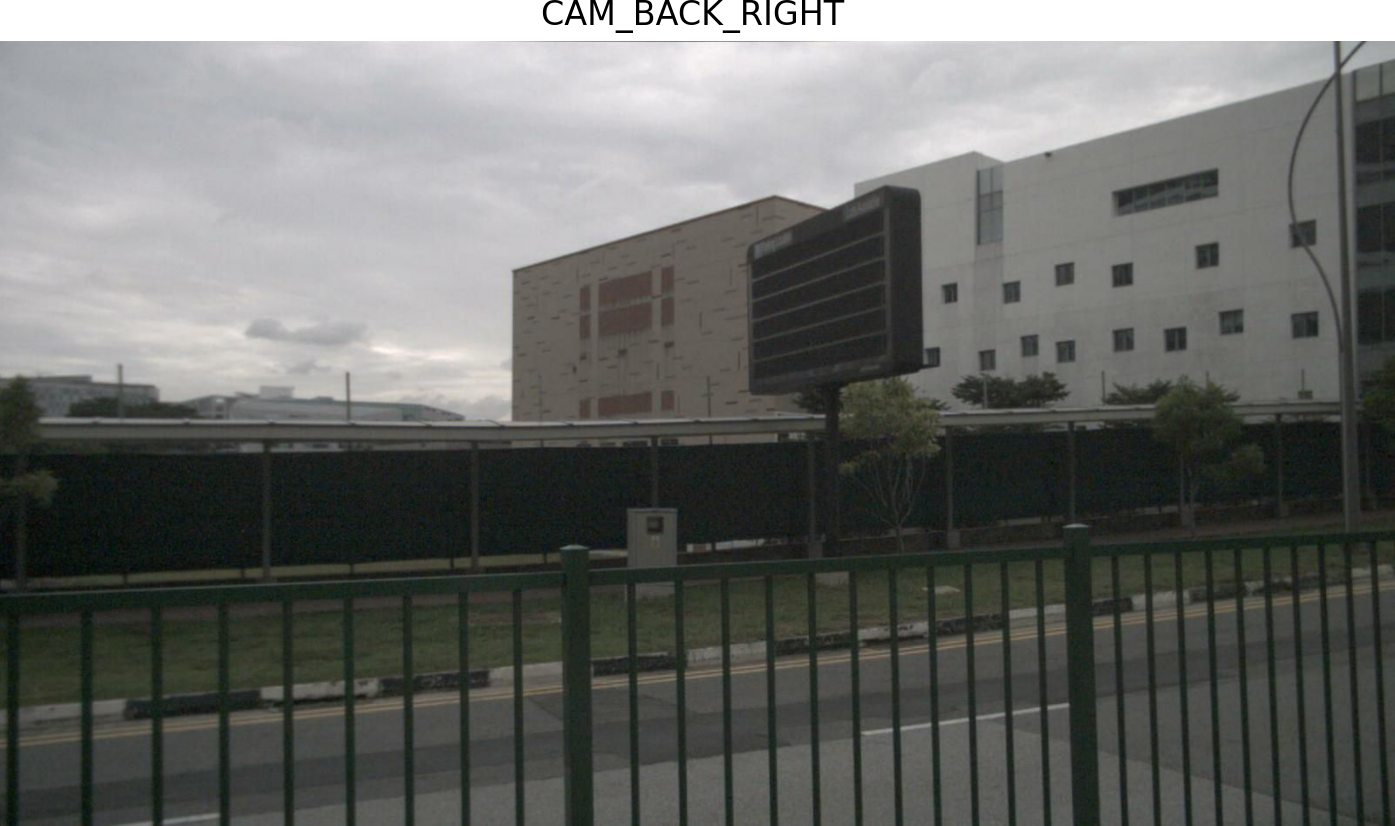
\includegraphics[width=0.31\columnwidth]{figure/visualize_predictions/CAM_BACK_RIGHT.png} \\ 
            \rotatebox{90}{\small{真值}} &
    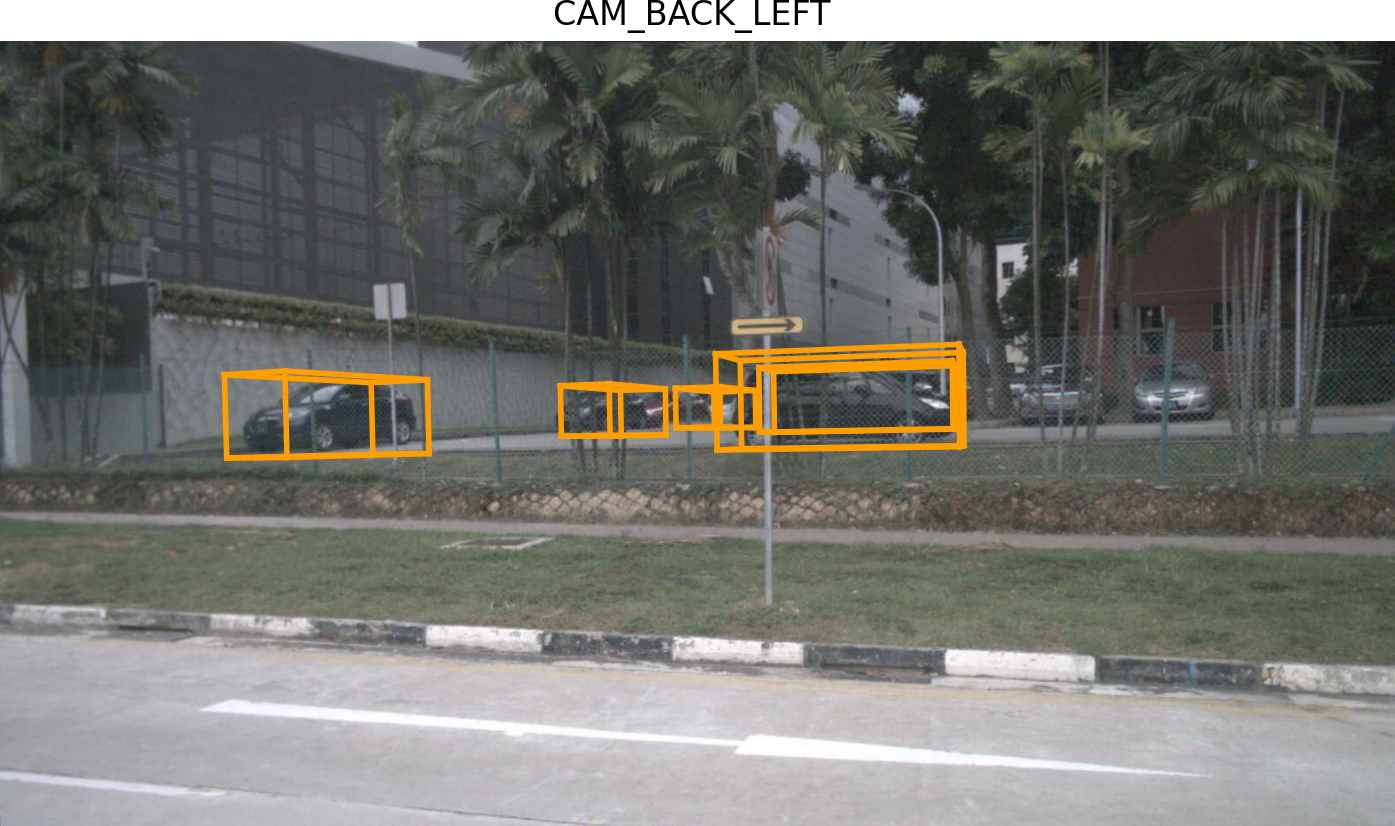
\includegraphics[width=0.31\columnwidth]{figure/visualize_predictions/GT-CAM_BACK_LEFT.png} & 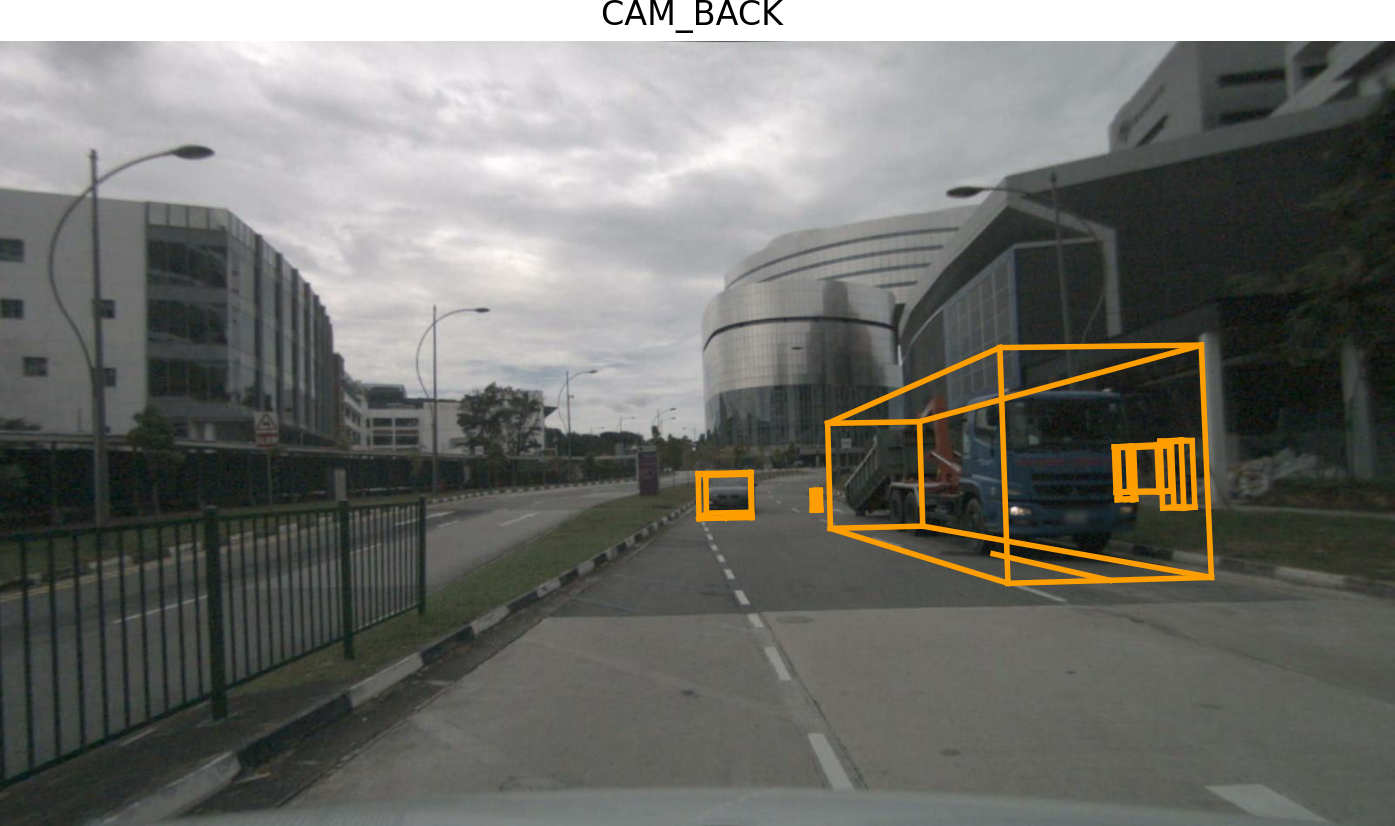
\includegraphics[width=0.31\columnwidth]{figure/visualize_predictions/GT-CAM_BACK.png} & 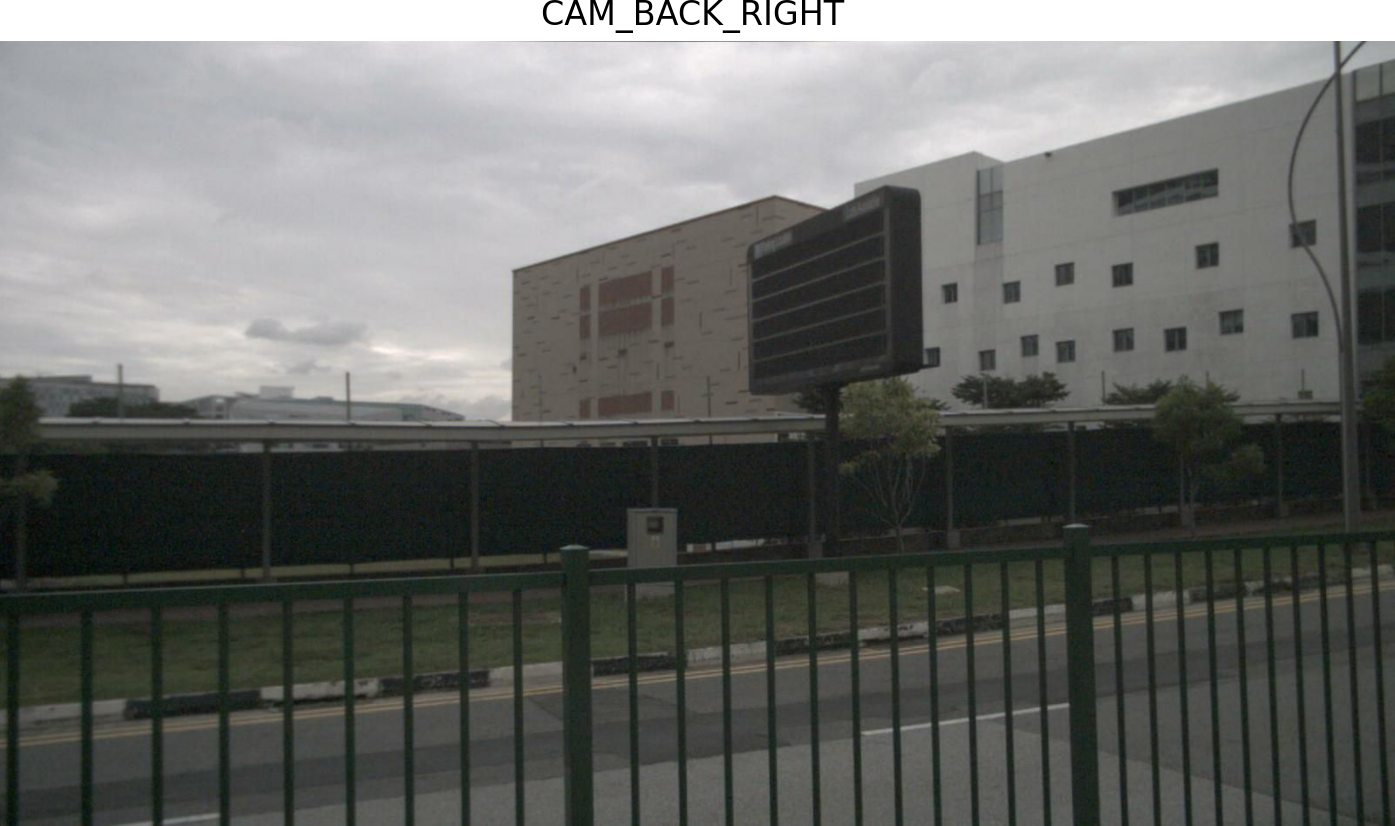
\includegraphics[width=0.31\columnwidth]{figure/visualize_predictions/GT-CAM_BACK_RIGHT.png} \\ 
    
        \end{tabular}
    \end{minipage} \\
    % \multirow{ 2}{*} 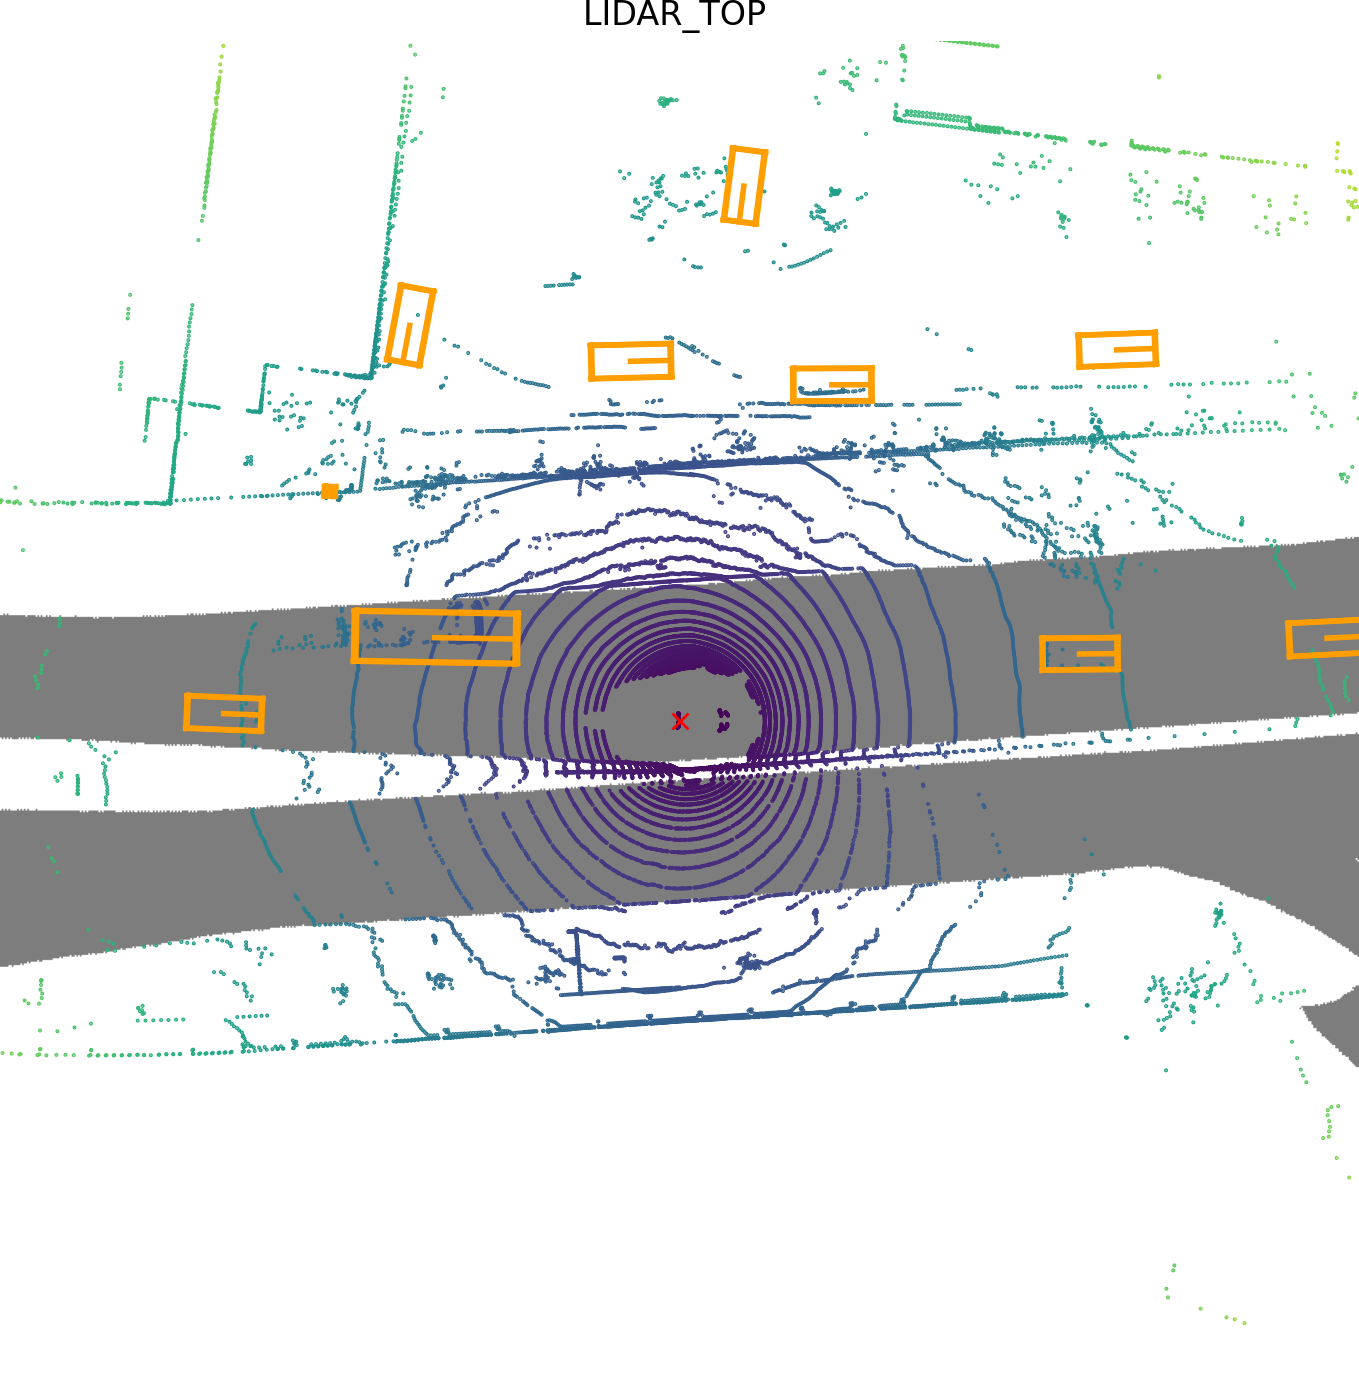
\includegraphics[width=0.3\columnwidth]{figure/visualize_predictions/LIDAR_TOP.png} & 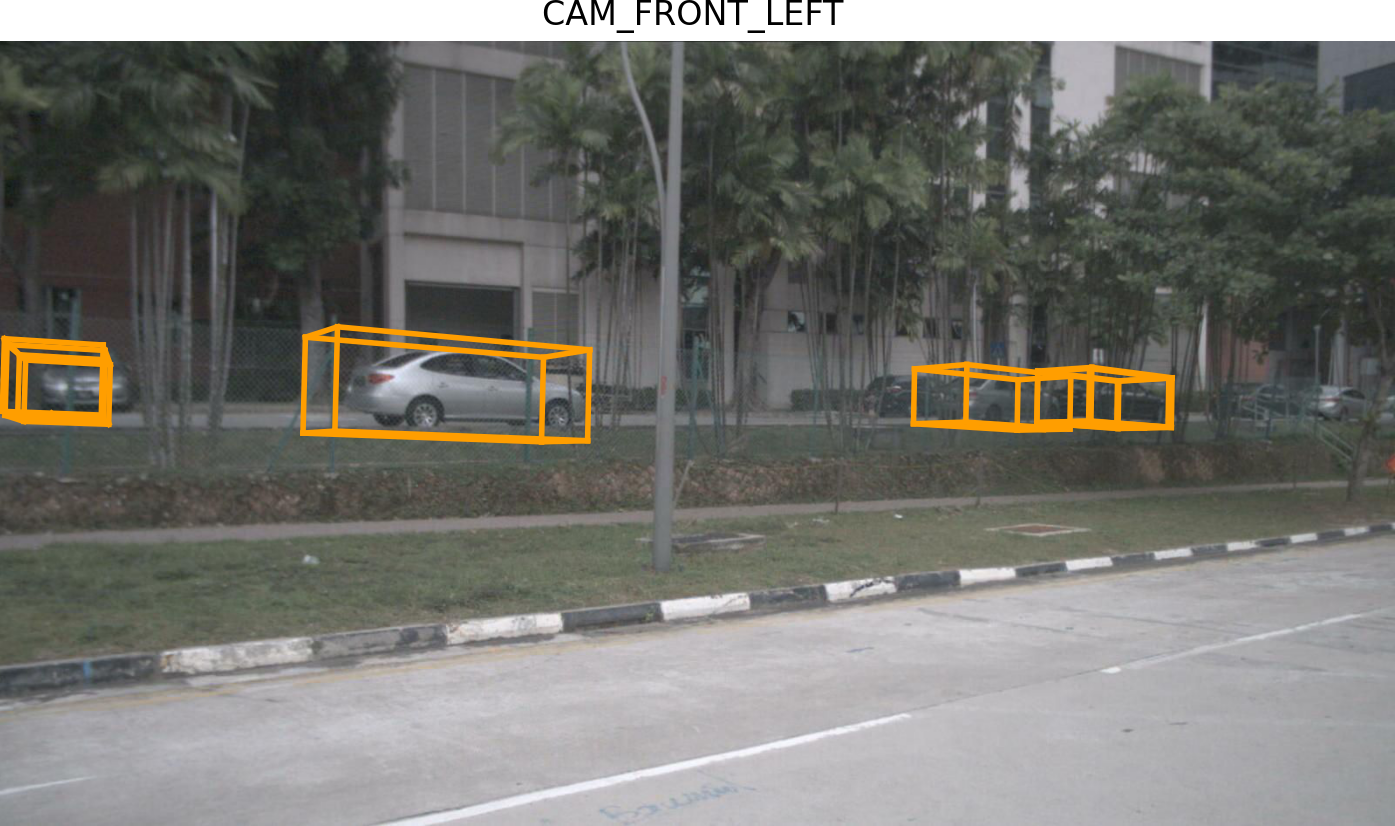
\includegraphics[width=0.3\columnwidth]{figure/visualize_predictions/CAM_FRONT_LEFT.png} & 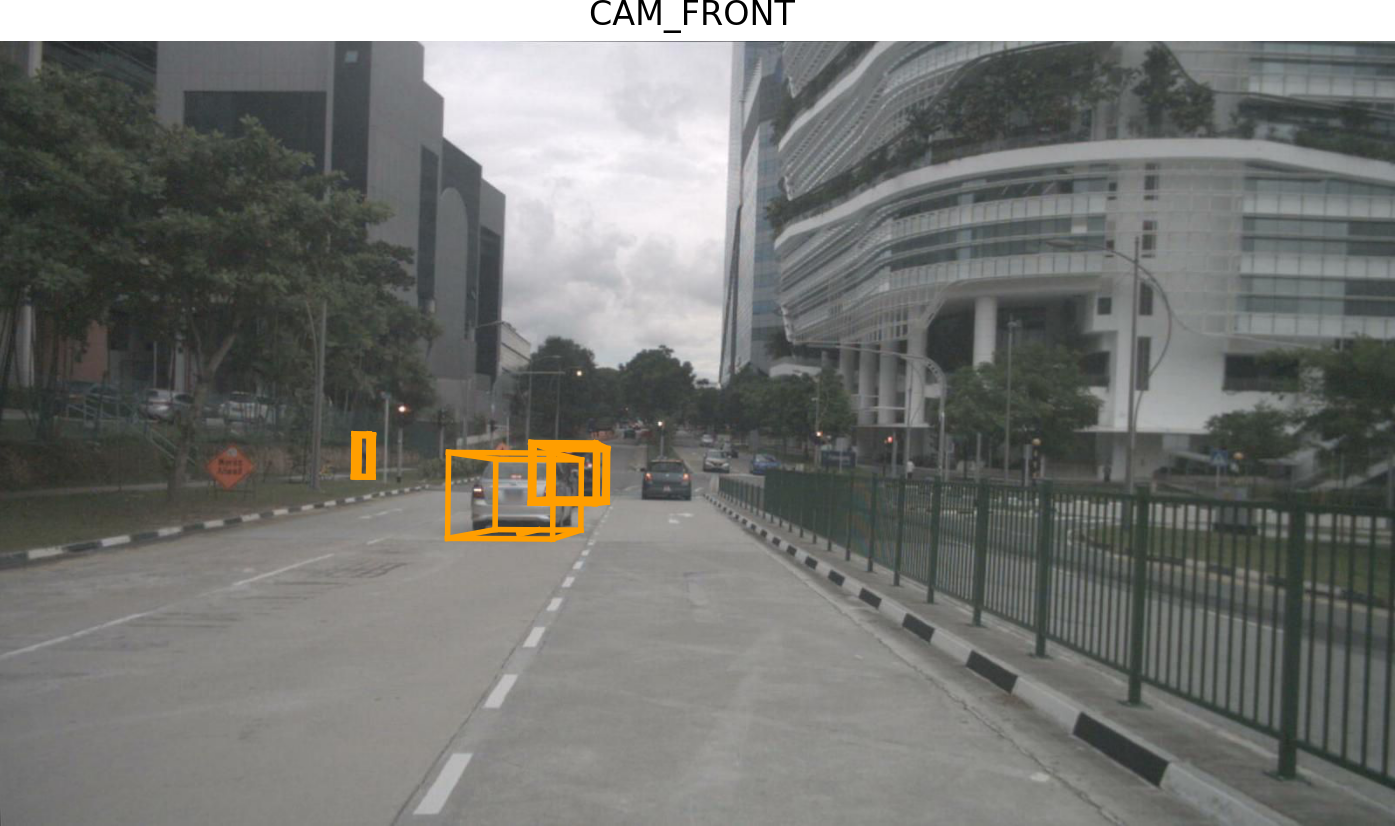
\includegraphics[width=0.3\columnwidth]{figure/visualize_predictions/CAM_FRONT.png} & 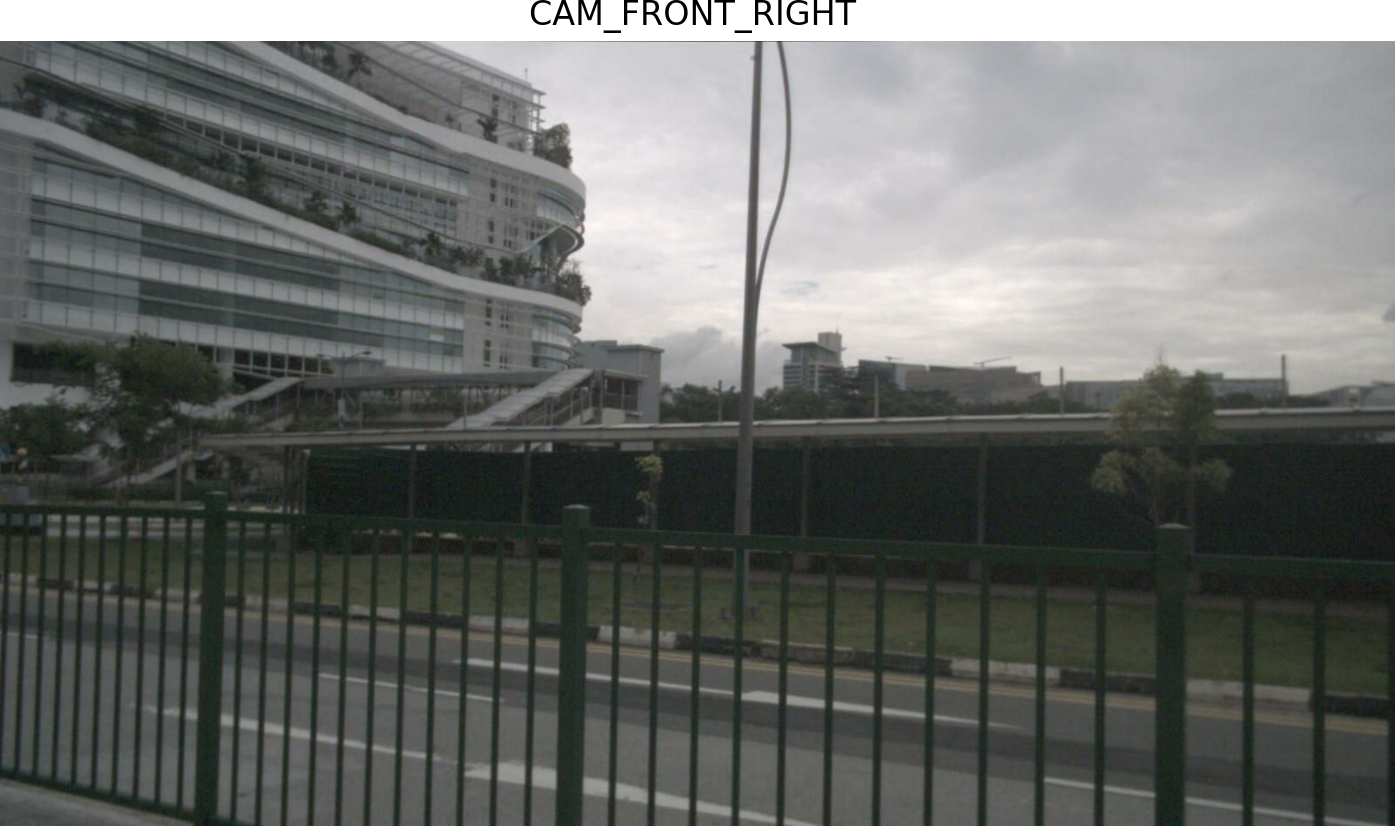
\includegraphics[width=0.3\columnwidth]{figure/visualize_predictions/CAM_FRONT_RIGHT.png} \\ 
    % & 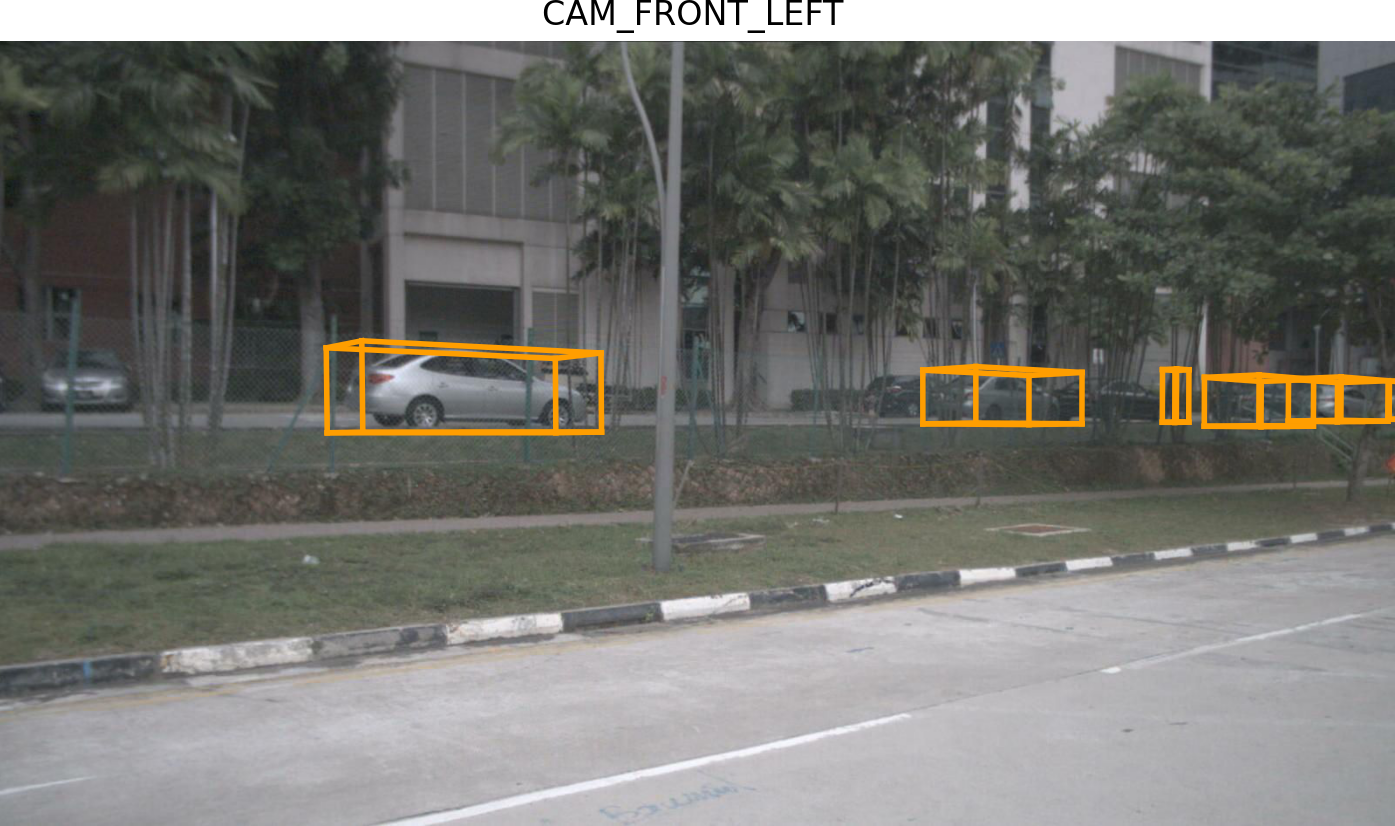
\includegraphics[width=0.3\columnwidth]{figure/visualize_predictions/GT-CAM_FRONT_LEFT.png} & 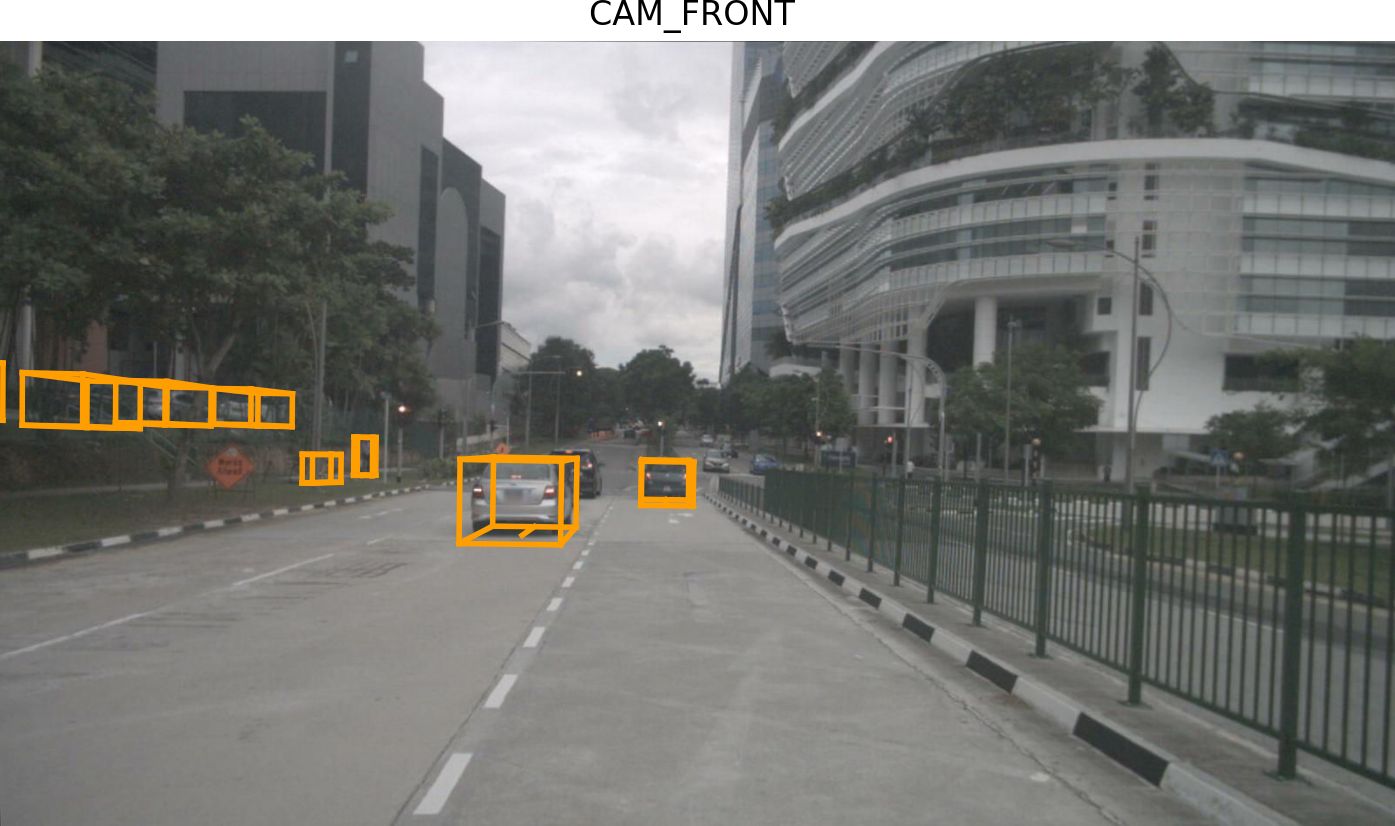
\includegraphics[width=0.3\columnwidth]{figure/visualize_predictions/GT-CAM_FRONT.png} & 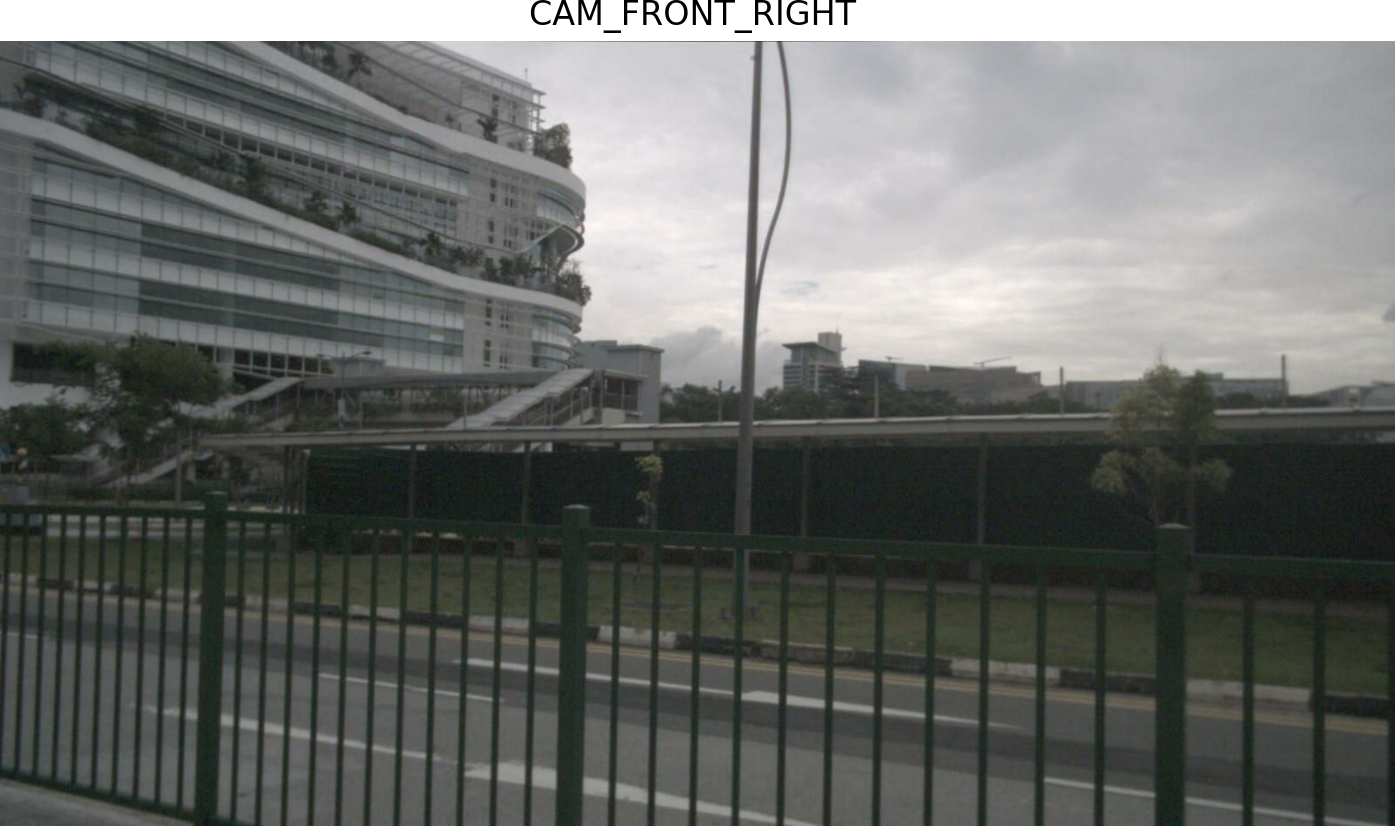
\includegraphics[width=0.3\columnwidth]{figure/visualize_predictions/GT-CAM_FRONT_RIGHT.png} \\ 
    \end{tabular}
  \caption{\name 预测结果的可视化，包括BEV和图像视图。本文模型能够检测相当小的目标，甚至包括未标注为真值的目标（\texttt{CAM\_BACK\_LEFT}中的车辆）。一些失败案例包括\texttt{CAM\_FRONT}中远处的车辆未被检测到。\label{fig:prediction}}
%   \vspace{-3em}
\end{figure}
% \end{comment}

%  Moreover, Table~\ref{sota} shows our method exhibits high translation error, which we suspect is due to the reference point parameterization; seeking better reference point parameterization can potentially increase the performance. 

% 1. Backbone of different sizes
% 2. Level, cam embedding


% Better Scene Prior: evaluate
% \begin{itemize}
%     \item Overlapping objects
%     \item What if one camera fails (low priority)
% \end{itemize}





% \subsection{Visualization}
% Visualize Ours backward
% \begin{itemize}
%     \item Reference points in 3d Scenes.  iterative refine process
%     \item Visualization feature fuse process (mask)
% \end{itemize}

% Visualization of Forward methods

% \begin{itemize}
%     \item Lift all pixels.
% \end{itemize}




\section{结论}

本文提出了一种解决从2D图像恢复3D信息这一不适定逆问题的新范式。在该设定下，输入信号缺乏必要信息，模型必须借助从数据中学习到的先验才能做出有效预测。其他方法要么仅在2D空间中进行计算，要么使用额外的深度网络重建场景，而本文方法在3D空间中操作，并通过反向投影按需获取图像特征。本文方法有两个优势：（1）消除了中间层表示（如预测的深度图或点云），这些表示可能成为累积误差的来源；（2）通过将同一3D点投影到所有可用帧，利用多相机信息。

除了直接应用于自动驾驶3D目标检测外，本文工作还有几个值得未来探索的方向。例如，单点投影在检索到的图像特征图中产生有限的感受野，为每个目标查询采样多个点将为目标优化融入更多信息。此外，新检测头与输入模态无关，引入激光雷达（LiDAR）/雷达（RADAR）等其他模态将增强性能和鲁棒性。最后，将本文流程推广到室内导航和物体操作等其他领域，将扩大其应用范围并揭示更多改进方向。 
%===============================================================================

\clearpage
% no \bibliographystyle is required, since the corl style is automatically used.
\bibliography{corl}  % .bib

% \clearpage

% \section*{Supplementary Material}
\subsection*{Comparison to FCOS3D without global NMS.}
We also compare our MVOD method to FCOS3D without global NMS. We test in both settings: benchmarking using all data and using ground-truth bounding boxes only in the overlap regions. As shown in Table~\ref{table:global-nms}, our model outperforms FCOS3D without global NMS. This suggests that FCOS3D is very reliant on global NMS, with a significant drop in performance when it is disabled, while our method completely eliminates the need for it. In addition, we also remove the per-image NMS in FCOS3D and the model fails. So we ignore the results in this table. 
%without global NMS, the performance of FCOS3D drops significantly while our model is robust to NMS. 

\begin{table}[t] 
\begin{center}
\caption{Comparisons to FCOS3D without global NMS. \label{table:global-nms}}
\resizebox{\linewidth}{!}{
\begin{tabular}{c|c|c|c|c|c|c|c|c|c}
\toprule
\hline
Method & NDS $\uparrow$ & mAP $\uparrow$ & mATE $\downarrow$ & mASE $\downarrow$ & mAOE $\downarrow$ & mAVE $\downarrow$ & mAAE $\downarrow$ & global NMS  & overlap region only \\
\hline
FCOS3D $\ddag$ & 0.273 & 0.133 & 0.890 & 0.274 & 0.593 & 1.093 & 0.176 & - & 
\checkmark \\
\hline
FCOS3D & 0.317 & 0.213 & 0.841 & 0.276 & 0.604 & 1.122 & 0.173 &  \checkmark & \checkmark \\
\hline 
\name (Ours)  &  0.356 & 0.231 & 0.825 & 0.280 & 0.400 & 0.863 & 0.223 & - & \checkmark \\
\hline
FCOS3D $\ddag$ & 0.336 & 0.234 & 0.830 & 0.268 & 0.558 & 1.361 & 0.153 & - & - \\
\hline
FCOS3D $\ddag$ & 0.373 & 0.299 & 0.785 & 0.268 & 0.557 & 1.396 & 0.154 & \checkmark & - \\
\hline
\name (Ours)  &  0.374 & 0.303 & 0.860 & 0.278 & 0.437 & 0.967 & 0.235 & - & - \\
\hline
\bottomrule
\end{tabular}
}
\end{center}
\end{table}

\subsection*{Time complexity.}
We compare the time complexity of FCOS3D with and without global NMS to that of our proposed MVOD model. Table~\ref{table:time-complexity} shows that MVOD is more efficient at inference time thanks to its NMS-free design. We also provide the performance when the NMS is not used in the FCOS3D. The per-image NMS contributes to a large portion of the overhead, which is not required by our model. 
We also note that further improvements in efficiency can be achieved by implementing more GPU-friendly feature sampling in our model. These frame rates were measured on a single Nvidia RTX 3090.

\begin{table}[t] 
\begin{center}
\caption{Time complexity.\label{table:time-complexity}}
 \vspace{-1.5em}
\resizebox{\linewidth}{!}{
\begin{tabular}{c|c|c|c|c}
\toprule
\hline
Models & FCOS3D & FCOS3D (w/o global NMS) & FCOS3D (w/o global NMS, w/o per-image NMS) & MVOD (ours)  \\
\hline
FPS & 1.1 & 1.2 & 3.3 & 3.1 \\
\hline
\bottomrule
\end{tabular}
}
\end{center}
\end{table}




\end{document}
